% =============================================================================
% UNL Dissertation Template
% Based on nuthesis.cls (Hummel & Dieter, 2013)
% Author: Joe Sandow, University of Nebraska-Lincoln
% Chapter 2: Do Guns Make Us Safe?
% =============================================================================

\documentclass{nuthesis}

% -----------------------------------------------------------------------------
% Required packages
% -----------------------------------------------------------------------------

% Font
\usepackage[sc,osf]{mathpazo}       % Palatino font, matches nuthesis example
\usepackage{microtype}              % Better typography
\renewcommand{\bf}{\bfseries}

% Math
\usepackage{amsmath}
\usepackage{amsfonts}
\usepackage{bbm}                    % for \mathbbm{1} indicator function

% Citations
\usepackage{natbib}

% Tables
\usepackage{booktabs}
\usepackage{threeparttable}         % For table notes
\usepackage{longtable}
\usepackage{tabularx}
\usepackage{multirow}
\usepackage{makecell}

% Figures
\usepackage{graphicx}
% Search tables/ and figures/ as well as the compile directory, so the same
% \input{table_x} and \includegraphics{fig_y} calls resolve whether the files
% sit beside this document or in the outputs/ tree pulled from the repo.
\graphicspath{{./}{figures/}{outputs/figures/}}
\makeatletter
  \def\input@path{{./}{tables/}{outputs/tables/}}
\makeatother
\usepackage{caption}
\usepackage{subcaption}
\usepackage{float}

% Layout
\usepackage{pdflscape}
\usepackage{rotating}
\usepackage{indentfirst}
\usepackage{paralist}
\usepackage{epigraph}

% TikZ (for diagrams if needed)
\usepackage{tikz}
\usetikzlibrary{trees,shapes,arrows,positioning}

% Fixes for memoir + hyperref compatibility
\usepackage{memhfixc}

% Hyperlinks (load last)
\usepackage{hyperref}
\hypersetup{
    colorlinks = true,
    linkcolor  = black,
    citecolor  = black,
    urlcolor   = black
}

\setlength{\footskip}{12pt}

% A second \def\input@path lived here and silently overrode the one set beside
% \graphicspath above, so \input resolved only against tables/ and figures/.
% Removed 2026-10-21; the definition above covers those plus ./ and the
% outputs/ tree, so the same calls work whichever layout the compile sees.
% =============================================================================
% Document metadata — UPDATE THESE FIELDS
% =============================================================================

\begin{document}

\frontmatter

\title{Mother of Exiles, Maker of Scholars: Immigrant Exposure and
       U.S.-born Educational Attainment}
\author{Joe Sandow}
\adviser{Professor [Edward Balistreri]}          % UPDATE
\adviserAbstract{[Edward Balistreri]}            % UPDATE (first and last name only)
\major{Economics}
\degreemonth{[December]}                       % UPDATE e.g. May
\degreeyear{[2026]}                         % UPDATE e.g. 2026

% =============================================================================
% Title page (auto-generated by nuthesis)
% =============================================================================

\maketitle

% =============================================================================
% Abstract (max 350 words including title, name, etc.)
% =============================================================================

\begin{abstract}

\noindent Existing work suggests that immigration leads less-educated
U.S.-born workers out of manual and into communication-intensive occupations.
Whether it also changes how much schooling adolescents and young adults
acquire is less well established. This paper estimates the effect of immigrant exposure during the
formative years on U.S.-born educational attainment, using repeated
cross-sections from the 1990--2023 census and American Community Survey across
the 175 largest metropolitan areas. National immigrant arrivals by origin are
allocated to metropolitan areas using 1990 settlement shares across 230 origin
groups; exposure is the predicted inflow averaged over each individual's ages
15 through 25, so treatment varies at the metropolitan-area by birth-cohort
level. A one standard deviation increase in exposure raises the probability of
completing high school or more by 4.74 percentage points, against a first stage
of 0.647. The effect works on whether secondary schooling is finished at all
rather than on how far beyond it an individual goes: those moved out of
no-high-school spread across the higher categories in the proportions already
observed there. Following \citet{card2001immigrant}, U.S.-born internal
migration does not respond to immigrant inflows, and occupation-specific wage
estimates show no detectable effect at the low-skill end while pointing to a
possible motivation for the additional schooling.

\end{abstract}

% =============================================================================
% Copyright page (optional)
% =============================================================================

\begin{copyrightpage}
% Auto-generates: Copyright © [year], [author]
% Leave blank or add text below if needed
\end{copyrightpage}

% =============================================================================
% Dedication (optional — delete environment if not needed)
% =============================================================================

\begin{dedication}
% e.g. To my family.
\end{dedication}

% =============================================================================
% Acknowledgments (optional — delete environment if not needed)
% =============================================================================

\begin{acknowledgments}
% Thank your adviser, committee, funding sources, etc.
\end{acknowledgments}

% =============================================================================
% Front matter tables
% =============================================================================

\tableofcontents
\listoffigures
\listoftables

% =============================================================================
% Main body
% =============================================================================

\mainmatter

% =============================================================================
% Chapter 2
\label{chap:immigration}
% =============================================================================
\chapter{Mother of Exiles, Maker of Scholars: Immigrant Exposure and U.S.-born Educational Attainment}
%{Immigrant Exposure During Formative Years and Native Educational Attainment: Shift-Share Evidence from U.S. Metropolitan Areas, 1990--2023}


\setlength{\epigraphwidth}{0.6\textwidth}

% =============================================================================
\section{Introduction}
\label{sec:immigration_intro}
% =============================================================================
\epigraph{
  \textit{Not like the brazen giant of Greek fame,\\
  With conquering limbs astride from land to land;\\
  Here at our sea-washed, sunset gates shall stand\\
  A mighty woman with a torch, whose flame\\
  Is the imprisoned lightning, and her name\\
  Mother of Exiles.}
}{--- Emma Lazarus, \textit{The New Colossus} (1883)}

Few forces (Lazarus's imprisoned lightning) shape the trajectory of a nation as fundamentally as immigration and education. The latter's influence on individual and aggregate economic outcomes is well documented; the former's is contested; and the interaction between them remains incompletely understood. Against a backdrop of heightened immigration enforcement and renewed political debate over the role of immigrants in American society, understanding the causal relationship between immigrant exposure and U.S.-born human capital formation is of both scholarly and practical urgency. \cite{hunt2017impact}, using a state panel spanning 1940--2010, finds that a one percentage point increase in the immigrant share of the population raises the probability that a U.S.-born American completes high school by 0.3 percentage points — a positive and statistically significant effect that motivates renewed inquiry into the mechanisms linking immigrant exposure to U.S.-born educational investment.

%When we think of potential ``imprisoned lightning(s)'' or powerful forces that impact our lives it is hard to come up with two as pervasive as immigration and education. The later, at least here in the US, is obvious the former less so, and the interaction betwixt them less so still though not wholly unknown. It is then natural given current events that we become curious if the relationship identified previously still holds. Using a state panel dataset \cite{hunt2017impact} found that a one percentage point increase in immigration rates lead to a 0.3 percentage point increase in the likelihood a U.S.-born American would graduate from high-school.  
%In 1980 Fidel Castro exiled over 100,000 mostly low-skilled young men from Cuba, they found refuge in Miami, an event that came to be called the Muriel Boat-lift. Studying that event Card produced a paper with a finding that went counter to basic economic theory, a positive supply shock had not decreased the price, the sudden increase in low-skilled labor had not depressed wages in Miami \cite{card1990impact}. 

This paper estimates the causal effect of immigrant inflow exposure during formative years on the educational attainment of U.S.-born adults. Using individual-level data from IPUMS USA spanning 1990--2023, the analysis constructs a shift-share instrumental variable following \cite{card2001immigrant} that predicts MSA-level immigrant inflows using historical national-origin settlement patterns. The instrument is averaged over each U.S.-born's ages 15--25 to produce an individual-level measure of formative-year exposure, addressing the endogeneity that arises when immigrants sort across MSAs in response to local labor demand conditions that independently affect U.S.-born educational investment. Averaging exposure over the ages 15--25 window captures the cumulative immigrant presence a U.S.-born encounters during the period when educational investment decisions are most consequential. Because a 25-year-old resident of Cincinnati in 2010 has experienced a different sequence of local immigrant inflows than a 15-year-old resident of the same city in the same year, this individual-level exposure measure introduces variation within MSA and year cells that MSA-level panel designs cannot exploit. 
The preferred specifications, estimated via linear probability models with MSA and year fixed effects and MSA-clustered standard errors, find that immigrant exposure during the formative years raises educational attainment at both margins examined. A one-standard-deviation increase in average predicted immigrant inflow during a U.S.-born individual's ages 15--25 raises the probability of completing high school or more by 4.74 percentage points, and the probability of completing some college or above by 3.47 percentage points. In the underlying units, the reduced-form coefficient on the high-school margin is $7.25 \times 10^{-6}$ (clustered standard error $7.34 \times 10^{-7}$), and the corresponding two-stage least squares estimate is $1.12 \times 10^{-5}$ ($1.50 \times 10^{-6}$); the first stage is $0.647$ ($0.105$), a $t$-statistic of $6.14$. These estimates are drawn from 8,537,597 U.S.-born observations in 175 stable MSAs, of which 3,484,287 carry non-zero exposure and therefore identify the coefficient; because the instrument varies only across metropolitan area and birth cohort, those observations take roughly 5,775 distinct instrument values nested within 175 clusters, and inference is governed by the cluster count rather than the observation count. Section~\ref{sec:immigration_robustness} restricts the sample to progressively older birth cohorts: dropping those that carry no exposure variation raises the estimate sharply, and restricting further to older cohorts brings it back to the magnitude of the preferred specification. Because exposure is assigned at the metropolitan-area by birth-cohort level, any influence operating at that level remains in the error term.

The remainder of the paper proceeds as follows. Section~\ref{sec:immigration_lit} situates this paper within the literature on immigration and U.S.-born labor market and educational outcomes, and engages directly with the methodological literature on shift-share identification. Section~\ref{sec:immigration_data} describes the data, the sampling design, and the descriptive patterns -- by education, origin country, and age at arrival -- that motivate the empirical design that follows. Section~\ref{sec:immigration_id} details the construction of the shift-share instrument and the individual-level exposure measure. Section~\ref{sec:immigration_results} presents the main estimation results, a brief and deliberately exploratory wage check by occupation group, and a Card (2001)-style replication check -- using both a direct shift-share instrument and a change-based instrument -- validating the assumption that immigrant inflows do not induce confounding native outflow. Section~\ref{sec:immigration_robustness} presents a series of robustness checks on the education specification, addressing cohort-trend confounds, the exposure\_missing indicator, MSA panel stability, and shift-share inference concerns, and Section~\ref{sec:immigration_conclusion} concludes with a discussion of the results and their implications.

%The preferred binary IV specifications, estimated via linear probability models with MSA and year fixed effects and MSA-clustered standard errors, find that a 100-person increase in average predicted immigrant inflow during a native's ages 15--25 raises the probability of high school completion relative to non-completion by 0.12 percentage points, the probability of college attendance relative to non-completion by 0.44 percentage points, and the probability of graduate degree attainment relative to non-completion by 0.15 percentage points. These effects are identified across 86 estimation samples drawn from 8.54 million observations in 175 stable MSAs, with a mean first-stage F-statistic of 215.5, well above conventional weak-instrument thresholds.
%This paper estimates the causal effect of average immigration exposure on the educational attainment of US born Americans. Using a repeated cross-sectional dataset from 1990--2023, the analysis employs a shift-share instrumental variable averaged over ten years in the top 175 MSAs to address any endogeneity between immigrant location choice of Metropolitan Statistical Area (MSA/Cities) and MSA level economic factors impacting US-born educational attainment. By averaging exposure over ten formitave years (15-25) this study is able to account for locational externalities down to the MSA level as a 25 year old in Cincinnati in 2010 will have a different immigration exposure then a 15 year old living in Cincinnati in 2010. The preferred two-way fixed effect specifications find that for a one percentage point increase in average immigration inflow exposure results in a 0.12 percentage point increase in the likelihood a US-born individual will reach 12 years of schooling over not completing high-school, a 0.44 percentage point increase in the likelihood of attending some college vs not completing high-school, and a 0.15 percentage point increase in likelihood that a US-born individual will complete some graduate work (or equivalent) over not completing high-school.

% =============================================================================
\section{Literature Review}
\label{sec:immigration_lit}
% =============================================================================

In 1980, the Cuban government permitted the emigration of approximately 125,000 Cuban nationals, the majority of whom settled in Miami in what came to be known as the Mariel Boatlift. Exploiting the Boatlift as a natural experiment, \cite{card1990impact} finds that the sudden influx of low-skilled labor had no discernible effect on the wages or employment of U.S.-born workers or earlier-arriving immigrants in Miami — a result at odds with the prediction of a standard competitive labor market model. This finding, together with \cite{card2001immigrant}'s result that immigrant inflows do not induce compensating outflows of U.S.-born workers from receiving MSAs, established an influential body of evidence suggesting that immigration imposes modest labor market costs on U.S.-born individuals. \cite{borjas2003labor} challenges this view directly, estimating that a 10 percent immigration-induced increase in labor supply reduces wages within a skill group by 3 to 4 percent — a finding that initiated a sustained empirical debate over the appropriate unit of analysis and the degree of substitutability between immigrant and U.S.-born workers. \cite{card2005new} challenges the Borjas framework, finding no impact of immigrant inflows on the relative wages of U.S.-born high school dropouts despite a strong cross-area correlation between differential immigrant inflows and the local supply of low-skilled U.S.-born workers — a discrepancy Card attributes to the endogenous geographic sorting of U.S.-born workers in response to immigration. \cite{borjas2006native} offers a partial reconciliation, demonstrating that U.S.-born internal migration responds to immigrant inflows — inmigration to receiving areas falls and outmigration rises — such that the local labor supply effect of immigration is partially offset by U.S.-born mobility, attenuating the wage impact observable in local labor markets. This debate over the magnitude of wage effects obscures a more fundamental question about the nature of immigrant-U.S.-born competition. \cite{card2009immigration} demonstrates that immigrant and U.S.-born workers are imperfect substitutes in production, implying that the competitive threat to U.S.-born wages is more limited than a homogeneous-labor framework suggests. \cite{peri2009task} provides the mechanism: U.S.-born workers hold a comparative advantage in communication-intensive tasks relative to similarly educated immigrants, and respond to immigrant inflows by reallocating toward those tasks rather than competing directly for the same positions.
%In 1980 Fidel Castro exiled over 100,000 mostly low-skilled young men from Cuba, they found refuge in Miami, an event known as the Muriel Boat-lift. From that natural experiment \cite{card1990impact} found that contrary to a simple positive supply shock leading to lower prices (wages) economic analysis, the Muriel Boat-lift did not lead to lower wages for US-born or earlier moving immigrant Miamians \citep{card1990impact}. This finding along with the \cite{card2001immigrant} finding that immigration inflows do not impact US-born outflows from MSAs touched off a series of response papers between Card and Borjas when \cite{borjas2003labor} showed that wages decrease by 3 to 4 percent commensurate to a 10 percent increase in the labor supply. Contradicted then in \cite{card2005new} which found that there was no impact on the relative wages of US-born high-school dropouts even though there is a strong corelation between differential immigrant inflows and the supply of US-born dropouts. Looking to explain the muted wage response for US-born individuals \cite{borjas2006native} found that in the presence of immigration US-born in- migration is lower and out- migration is higher constituting a decrease in the growth rate of the US-born labor-force. All of which culminated in 2009 with the duel findings that immigrants and US-born workers are imperfect substitutes \citep{card2009immigration}, and as such they may act as more complimentary workers instead of substitutes \citep{peri2009task}.

The task reallocation documented by \cite{peri2009task} raises a natural subsequent  question: through what mechanism do U.S.-born workers acquire the skills in communication-intensive work that enable this occupational sorting? One testable hypothesis is that U.S.-born workers respond to immigrant inflows by investing more heavily in education — upgrading their human capital precisely because the returns to communication-intensive work, which requires higher and more varied levels of schooling, have increased. A nascent but accelerating empirical literature examines this hypothesis directly. Before turning to that evidence, \cite{chiswick2004educational} offer an instructive finding from the immigrant side of the ledger: individuals who immigrate during their teenage years attain significantly fewer years of schooling than those who arrive at pre-teen or post-teen ages, establishing that the years spanning approximately ages 15 through 25 constitute a sensitive period for educational investment. By analogy, if the arrival of immigrants disrupts the educational trajectories of the immigrants themselves during these years, exposure to that arrival may similarly shape the investment decisions of the U.S.-born students who share schools and labor markets with them.

%through what mechanism do U.S.-born workers acquire the communication-intensive skills that enable this occupational sorting?

%\cite{peri2009task} demonstrate that US born indivduals when faced with an influx of similiarly skilled immigrant labor will sort into more communication-intensive jobs leading to migrate labor being complimentary to US Born labor. This raises the natural question of how do the US born select into those communication-intensive jobs? One natural and testable hypothesis is that they do so through education, there is a nascent but accelerating literature addressing this question.Further \cite{chiswick2004educational} demonstrate that the timing of immigration matters critically for educational outcomes — individuals who immigrate during their teenage years attain significantly less schooling than those arriving at younger or older ages — suggesting that the ages 15 through 25 represent a formative window during which exposure to immigrant peers may shape educational investment decisions for U.S.-born students as well. Thus \cite{chiswick2004educational} add some nuance to the question we identified from \cite{peri2009task}, how and how soon do US born individuals begin to sort into communication-intensive occupations.

Despite its importance, the empirical literature on immigration and U.S.-born educational attainment remains comparatively thin relative to the voluminous literature on immigration and U.S.-born labor market outcomes. For much of the post-1980 period, the educational consequences of immigrant exposure for U.S.-born students were treated as a secondary concern, subordinate to the more immediately measurable question of wage and employment effects. The earliest systematic contributions, \cite{betts1998educational} and \cite{hoxby1998immigrants}, appeared not as standalone journal articles but as chapters in an edited volume examining the economic implications of immigration for African Americans — a framing that reflects the peripheral status the question then occupied in the literature. Both papers examined whether immigrant enrollment crowded U.S.-born minority students — particularly African Americans — out of educational opportunities. \cite{betts1998educational} finds some evidence of a negative relationship, with immigrant inflows reducing high school completion rates among Black and Hispanic U.S.-born students, while \cite{hoxby1998immigrants} finds little evidence of systematic displacement for the typical U.S.-born student. The crowding-out question was revisited by \cite{betts2003immigration}, who find that immigrant enrollment in public secondary schools induces a significant behavioral response among U.S.-born families: for every four immigrants who enter a public school, approximately one U.S.-born student transfers to a private school — a pattern the authors term native flight. Extending the native flight hypothesis to higher education, \cite{borjas2004foreign} finds that at the aggregate level there is little evidence that foreign students displace U.S.-born graduate enrollment, but documents a strong negative association between foreign student enrollment and the enrollment of white U.S.-born men — an effect concentrated at elite institutions and strongest in programs with the highest foreign student shares.

%Admitatedly the literature on immigration and US born educational attainment is thin relative to the enormous literature on immigration and US born labor market outcomes. The question of immigration and US born educational attainment was arguably viewed as peripheral to the labor market outcomes question. The foudnational papers \cite{betts1998educational, hoxby1998immigrants} offered mixed results, and were not published in stand alone journal articles instead they were chapters in a book on the imapcts of Immigration on African-Americans. And the question they were focused on was if immigrates crowded out African-Americans and other minorities \cite{betts1998educational} finds some evidence for a negative relationhip, while \cite{hoxby1998immigrants} finds little evidence. This question of crowding out would be revisted. \cite{betts2003immigration} finds that for secondary school students there was a large impact on the school choice between public or private of US born students. For every four immigrant students that enter public school one US born student would transfer to a private school \citep{betts2003immigration}. Extending the idea of crowding-out (or native flight) into college and more specifically graduate school, \cite{borjas2004foreign} finds little evidence that immigrants crowd out the typical student, but there is a strong negative association for white male graduate students.

The peer effects channel implicit in \cite{betts1998educational} receives more rigorous empirical treatment in \cite{gould2009immigration}, who exploit the mass migration wave from the former Soviet Union to Israel in the early 1990s to identify the causal effect of immigrant concentration in elementary school on the long-run academic outcomes of Israeli students. The scale and concentration of that immigration wave — nearly 20 percent of Israel's population within a decade — provides identifying variation analogous to the Mariel Boatlift in the U.S. context, with the additional advantage of administrative panel data tracking individual students from elementary school through high school completion. \cite{gould2009immigration} find that a 10 percentage point increase in the immigrant concentration in fifth grade lowers an Israeli student's probability of passing the high school matriculation examination by 1.5 to 1.8 percentage points, with adverse effects concentrated among students from disadvantaged socioeconomic backgrounds. Extending the peer effects framework beyond a single country, \cite{brunello2013effect} use aggregate PISA data spanning 19 countries over the period 2000--2009 and find a negative and statistically significant relationship between the share of immigrant pupils in secondary schools and the test scores of native students, though the estimated effect is small in magnitude. \cite{brunello2013effect} further demonstrate that, conditional on the average share of immigrant pupils, reducing the concentration of immigrant students across schools generates small but positive effects on native student performance: how immigrant pupils are spread across schools matters beyond their average share. The same consideration carried across time rather than across schools motivates the exposure measure used here. Averaging immigrant inflow exposure over each U.S.-born individual's ages 15--25 measures the immigrant presence a person encounters across the whole formative period rather than in the year they happen to be observed.

%It isn't until \cite{gould2009immigration} find better supported evidence for adverse effects for U.S.-born populations via peer effects that an implication from \cite{betts1998educational} is returned to and tested. It also points to the question we are attempting to answer even if the question in the paper is in a larval form, and albeit for Israel in the 90s. The large immigration waves into Israel during the 90s do provide a nice natural experiment much like the Muriel Boat lift did here in the states. Taking the peer effects approach and expanding it even further beyond Irael \cite{brunello2013effect} find a negative relationship between immigration and PISA test scores in 19 countries. Further \cite{brunello2013effect} show that reducing the dispersion of the share of immigrant students between schools has small positive effects of the U.S.-born born population. Hinting that average exposure to immigration flows may matter more than intesive exposures.

Returning to the U.S. context, \cite{mchenry2015immigration} provides an important empirical predecessor to the present study. Using the 1988 National Education Longitudinal Study linked to U.S. Census data and exploiting variation in immigration across Commuting Zones, McHenry finds that low-skilled immigration to a local labor market induces U.S.-born workers in that market to attain more years of schooling and shift toward more communication-intensive occupations — confirming the task reallocation mechanism identified by \cite{peri2009task} and establishing a positive causal link between immigrant inflows and U.S.-born human capital investment. The closest antecedent to the present study is \cite{hunt2017impact}, who uses decennial census data from 1940--2010 to construct a state panel examining the effect of the immigrant share of the population on U.S.-born high school completion rates. Instrumenting for the immigrant share using 1940 state settlement patterns across 18 source regions and countries, \cite{hunt2017impact} finds that a one percentage point increase in the share of immigrants among the population aged 11--64 raises the probability that a U.S.-born individual aged 11--17 eventually completes 12 years of schooling by 0.3 percentage points. The present study extends this line of inquiry in three respects. First, it resolves the instrument more finely across origins, distinguishing 230 origin groups from a 1990 base rather than 18 source regions. Second, it constructs an individual-level exposure measure averaged over each U.S.-born individual's ages 15--25, capturing the cumulative immigrant inflow experienced during the precise years when educational investment decisions are made. Third, it examines the full distribution of educational attainment — from high school completion through graduate degree attainment — rather than the binary high school completion margin alone.

\cite{costas2023effect} and \cite{figlio2024diversity} together sharpen the contrast between the educational effects of immigration observed in other countries and those documented in the U.S. context. \cite{costas2023effect} find that foreign students in English universities have zero to mild effects on the graduation probability and degree classification of British-born students at the aggregate level, though significant displacement effects emerge across institutions and degree types. Taken together with the small negative PISA effects documented by \cite{brunello2013effect} across 19 countries and the adverse effects on Israeli students found by \cite{gould2009immigration}, the international evidence presents a notably different picture from that emerging in the U.S. — suggesting that the positive relationship between immigrant exposure and U.S.-born educational attainment is specific to features of the U.S. labor market, most plausibly the language-based comparative advantage in communication-intensive occupations identified by \cite{peri2009task}. Within the U.S. context, earlier evidence suggested that marginalized populations bear a disproportionate share of any negative effects: \cite{betts1998educational} finds that immigrant inflows reduce high school completion among Black and Hispanic U.S.-born students, while \cite{hoxby1998immigrants} finds evidence of displacement from higher education. However, \cite{hunt2017impact} finds a positive effect of immigration on high school completion specifically for Black U.S.-born individuals — a result that calls into question whether the negative effects documented in the late 1990s persist across the longer panel. The individual-level structure of the data in the present study would permit a heterogeneity analysis across racial and socioeconomic groups. However, although race indicators are included as controls in all specifications, a full heterogeneity analysis by racial group is precluded by the sparsity of parental education records for certain subpopulations in the IPUMS data and the resulting collinearity these variables introduce in the estimation. This limitation points toward the frontier of the literature. \cite{figlio2024diversity} address the parental background data problem directly by using population-level administrative birth and school records from Florida, enabling both longitudinal tracking of individual students and complete parental background information. Their findings document a positive effect of immigrant peers on U.S.-born student academic performance — among the most credible causal evidence yet available. However, this methodological strength comes at the cost of geographic scope: Florida, while a high-immigration state, may not be representative of the full range of MSA-level immigrant exposure dynamics observed nationally. While \cite{figlio2024diversity} exploit population-level administrative records to track individual students longitudinally within a single state, the present study uses repeated cross-sections from IPUMS USA spanning 175 MSAs nationally from 1990--2023, constructing individual-level variation in immigrant exposure from differences in birth cohort and MSA of residence rather than from longitudinal observation. This design enables a broadly representative study across U.S. metropolitan areas of the full education distribution across three decades, at the cost of the individual longitudinal tracking that administrative records permit — a tradeoff that future work with national administrative data could resolve.

This same design choice — repeated cross-sections rather than longitudinal administrative panels — is what necessitates an instrumental variables strategy to isolate the causal effect of immigrant exposure from the many other factors that vary across birth cohorts and metropolitan areas. The shift-share instrument constructed for this purpose belongs to a class of research designs that has itself become the subject of substantial methodological scrutiny in recent years, and establishing the credibility of the paper's findings requires engaging directly with this literature. This style of instrument originates with \citet{bartik1991benefits}, who constructs a shift-share instrument to isolate exogenous local labor-demand shocks from a region's initial industry composition, and is adapted specifically to the immigration setting by \citet{altonjicard1991effects}, who instrument for the contemporaneous immigrant share of a labor market using the historical settlement pattern of earlier immigrant cohorts by origin country -- the same logic underlying the instrument constructed in the identification section below.

\cite{goldsmith2020bartik} establish that any shift-share estimator can be written as a weighted average of just-identified instrumental variables estimators, one for each ``share'' -- in this application, one for each origin country -- with weights (Rotemberg weights) summing to one and determined by each share's relative contribution to the first stage. The validity of a shift-share design rests on the exogeneity of those shares with non-trivial weight, so a design in which a small number of shares carry the bulk of identifying variation is only as credible as the exogeneity argument for those specific shares. The decomposition reported in Section~\ref{sec:immigration_id} finds moderate concentration by the standards of the applications \cite{goldsmith2020bartik} survey, and -- more to the point -- an estimate that is close to unmoved by removing the origins carrying the most weight. Excluding the single largest origin changes the point estimate by 3.3 per cent, and excluding the ten largest, which together account for more than half of the identifying weight, changes it by 4.5 per cent. The origin-specific estimates are themselves dispersed -- the ten highest-weighted origins return just-identified estimates spanning roughly a factor of two -- but they share a sign and a magnitude, so the pooled estimate is an average over genuinely heterogeneous effects rather than a result sustained by any one share.


A second concern, raised by \cite{adao2019shift}, is that shift-share instruments constructed from a common set of national-level shocks induce correlation in the implicit regression residuals across regions exposed to similar shock compositions, a form of cross-sectional dependence that conventional region-clustered standard errors may fail to capture, potentially understating the true sampling variability of the estimate. \cite{adao2019shift} recommend a placebo-based diagnostic: if MSA-clustered standard errors understate true variability due to this mechanism, then placebo outcomes that are mechanically unrelated to the instrument should nonetheless exhibit inflated test statistics under MSA clustering relative to a coarser clustering scheme such as by state. Section~\ref{sec:immigration_id} applies this diagnostic to three placebo outcomes determined at birth. Two show no significant relationship with the instrument under either clustering scheme. The third, an indicator for Asian identity, is significant under both, reflecting the correlation between Asian population shares and the shift-share instrument in the gateway metropolitan areas where Asian immigration has historically concentrated; it is a limitation of the design. Most directly relevant to the main result, the state-clustered standard error on the headline two-stage least squares estimate is smaller than the MSA-clustered standard error, a ratio of 0.880 — direct evidence that, for the estimate of primary interest, MSA clustering is the more conservative choice and that the cross-sectional dependence \cite{adao2019shift} describe does not appear to be inflating the reported significance of the paper's central finding.

A third strand of this literature, \cite{borusyak2022quasi}, reframes the identifying assumption of shift-share designs in terms of the exogeneity of the underlying national-level shocks — here, annual national immigration inflows by origin country — rather than the exposure shares themselves, and notes that the effective sample size relevant for inference is determined by the number of shocks rather than the number of individual-level observations. Two features of the present design bear on that framework. The first is that its shock dimension is annual rather than decennial: the national inflow series is reconstructed from each immigrant's self-reported year of arrival rather than from the survey calendar, across the 230 origin regions entering the estimation.\footnote{The extract records 254 distinct birthplace codes among the foreign-born, of which 248 are foreign countries and the remainder are US territories or residual categories such as ``Abroad, n.s.'' and ``At sea.'' The 230 reported here are those entering the estimation: an origin qualifies if it has either a non-zero 1990 settlement share across the 175 metropolitan areas or recorded arrivals within the exposure window, and 230 satisfy at least one. Of these, 226 have a 1990 share and 148 have both, the latter being the set that can carry non-zero weight in the Rotemberg decomposition reported in Section~\ref{sec:immigration_id}.} The second is that the exposure shares follow \citet{card2001immigrant} and do not sum to one within a metropolitan area, which places the design in what \cite{borusyak2022quasi} term the incomplete-shares case and calls for a specific control. Section~\ref{sec:immigration_id} takes up both, and reports that control in Table~\ref{tab:bhj_incomplete_shares}.

Finally, \cite{jaeger2018shift} demonstrate that because immigrant settlement patterns exhibit substantial persistence over time, a contemporaneous shift-share instrument risks conflating short-run and long-run labor market responses, since the predicted immigrant inflow in any given year is correlated with inflows in prior years to which the local labor market may have already partially adjusted. The individual-level exposure measure constructed for the present study — the average shift-share predicted immigrant inflow experienced during the years each U.S.-born individual was aged 15 to 25, computed for all individuals whose age-25 year falls in 2000 or later — is, by construction, a measure of cumulative exposure over a decade-long window rather than a single contemporaneous shock, and is therefore conceptually aligned with the longer adjustment horizon \cite{jaeger2018shift} argue is necessary for valid inference in this setting. Moreover, because the outcome of interest — educational attainment — is itself the product of a cumulative, long-run investment decision rather than a contemporaneous labor market outcome such as wages or employment, the mismatch between instrument timing and outcome timing that motivates the \cite{jaeger2018shift} critique in short-run labor market applications is, by the structure of the present design, considerably less applicable.

Taken together, this literature leaves open a well-defined gap that the present study is designed to fill. The labor market literature establishes that U.S.-born workers respond to immigrant inflows through occupational reallocation rather than displacement \citep{card2009immigration, peri2009task}, but says little about the human capital investment margin -- whether and how U.S.-born individuals adjust their educational attainment in anticipation of, or in response to, that reallocation. The nascent literature on immigration and U.S.-born educational attainment has begun to answer this question, but existing U.S. evidence is either dated and narrowly focused on crowding-out among specific subpopulations \citep{betts1998educational, hoxby1998immigrants, betts2003immigration, borjas2004foreign}, or -- in the case of the closest available antecedent \citep{hunt2017impact} -- estimated at the state level using a high-school-completion outcome. This study extends that literature along three dimensions simultaneously: it resolves the instrument across 230 origin groups from a 1990 base rather than the 18 source regions available to \citet{hunt2017impact}, it constructs an individual-level exposure measure tied to each U.S.-born individual's own ages 15--25 rather than a contemporaneous area-level share, and it estimates at both the high-school and the college margin, decomposing the result across all four attainment categories to establish which margin the effect operates on. It further departs from \citet{figlio2024diversity}'s use of population-level administrative data restricted to a single state by drawing on repeated cross-sections spanning 175 MSAs nationally over three decades, trading individual longitudinal tracking for national representativeness. Finally, because this design relies on a shift-share instrument, the paper engages directly with the methodological literature examining when such designs are credible \citep{goldsmith2020bartik, adao2019shift, borusyak2022quasi, jaeger2018shift}, subjecting the instrument to a battery of diagnostics -- a Rotemberg decomposition, a placebo-outcome test under alternative clustering schemes, the sum-of-shares control an instrument built from incomplete shares requires, and a birth-cohort robustness check -- rather than assuming its validity is inherited from its use in earlier applications.

%\cite{costas2023effect} and \cite{figlio2024diversity} go to sharpen the contrast between immigration in other nations and the US particularly in regrads to the incumbent populations educational responces. \cite{costas2023effect} show a null result in higher education within English universities. That taken with \cite{brunello2013effect} slight negative PISA effects across 19 countries and \cite{gould2009immigration} negative results for Israeli students offers a contrast to what is seen in the US. Although there is evidence that mariginalized populations in the US do suffer negative impacts from immigration \cite{betts1998educational} and \cite{hoxby1998immigrants} this evidence is older and may no longer hold, as \cite{hunt2017impact} shows a positive impact for blacks. The individual-level structure of our data could allow for a heterogeneity analysis and although race indicators are included as controls in all specifications, a full heterogeneity analysis by racial group is precluded by the sparsity of parental education records for certain subpopulations in the IPUMS data and the resulting collinearity these variables introduce in the estimation. This limitation is acknowledged and left for future work with richer administrative data. \cite{figlio2024diversity} do have richer administrative data but as is usually the case this richer data comes at the cost of generality in that their data comes from floridia a high immigration state. The current study sacrificies specificity for generality. While \cite{figlio2024diversity} exploit population-level administrative records to track individual students longitudinally within Florida, the present study uses repeated cross-sections from IPUMS USA spanning 175 MSAs nationally from 1990--2023, constructing individual-level variation in immigrant exposure from differences in birth cohort and MSA of residence rather than from longitudinal observation. This allows for a national study, but does suffer  

%Returning to the U.S. context, \cite{mchenry2015immigration} provides an important empirical predecessor to the present study. Using the 1988 National Education Longitudinal Study linked to U.S. Census data and exploiting variation in immigration across Commuting Zones, McHenry finds that low-skilled immigration to a local labor market induces U.S.-born workers in that market to attain more years of schooling and shift toward more communication-intensive occupations — confirming the task reallocation mechanism identified by \cite{peri2009task} and establishing a positive causal link between immigrant inflows and U.S.-born human capital investment. Which leads to \cite{hunt2017impact} which uses the decennial census data from 1940-2010 as a state panel to look at the effect of the immigrant share of the population on the US-born high school completion. \cite{hunt2017impact} uses a shift-share based on continental origin groups, to find that an increase in the share of immigrates within the population of those 11-64 years of age leads to a 0.3\% increase in the probability that a US-born individual aged 11-17 completes 12 years of schooling. This study uses individual level data to estimate the impacts of average immigrant flows on the educational attainment of US-born individuals aged 15--25.

% =============================================================================
\section{Data}
\label{sec:immigration_data}
% =============================================================================

The analysis uses IPUMS USA data drawn from the decennial census in 1990 and 2000, combined with the American Community Survey (ACS) for every year from 2006 through 2019 and from 2021 through 2023. The 2020 wave is deliberately excluded: the Census Bureau's own documentation acknowledges that pandemic-era data collection for the 2020 ACS departed from standard sampling procedures, and rather than introduce a year of uncertain comparability into a panel that otherwise spans three decades of consistent design, it is omitted entirely. This leaves 19 sample years spanning 1990--2023, drawn from an initial pooled extract of roughly 80 million observations. The ACS is a 1 percent sample of the population in each surveyed year. The decennial census is available at either a 1 percent or a 5 percent sampling rate for 1990 and 2000, but because the identification strategy depends on metropolitan-area geographic detail, and in those two years that detail is carried by the 5 percent files and not the 1 percent ones, the analysis is restricted to the 5 percent files. To avoid introducing a sampling-rate inconsistency across years -- which would otherwise leave 1990 and 2000 sampled five times as densely as every ACS year -- a 20 percent random subsample is drawn of the 5 percent decennial files for 1990 and 2000, yielding an effective 1 percent sampling rate consistent with the ACS years.

Following \citet{card2001immigrant}, the extract retains all immigrants in the resulting extract along with a random 25 percent sample of U.S.-born individuals. This yields 7,154,407 immigrant observations (35.6 percent of the analysis sample) and 12,922,367 U.S.-born observations (64.4 percent), for a combined sample of 20,076,774. Table~\ref{tab:extract_composition} reports this composition, alongside the same breakdown for the age 25 and over sample used for the descriptive statistics later in this section. By design, immigrants are consequently overrepresented relative to their roughly 13--14 percent share of the U.S. population at large. This is intentional rather than a limitation: immigrants are the minority population of central interest, and full representation is necessary to construct the shift-share instrument and the actual-inflow measures with adequate precision, whereas U.S.-born individuals are the majority group whose role in the individual-level IV regressions is primarily as the outcome population, for which a 25 percent sample is more than sufficient.

The sample is further restricted to the 175 largest metropolitan statistical areas (MSAs) by population. Because the sample period spans more than three decades, the set of the 175 largest MSAs fluctuates somewhat from year to year as metropolitan areas grow, shrink, or newly qualify; taking the largest 175 MSAs independently in each year would therefore yield a different panel of metropolitan areas in every wave. To construct a single, stable set of MSAs for the full panel instead, the number of sample years in which each MSA appears among the top 175 is counted, and the 175 MSAs appearing most frequently across the panel are retained. A stable panel is a substantive requirement of the identification strategy rather than a matter of convenience: because identification relies on variation within MSA and within year net of MSA and year fixed effects, a metropolitan panel whose composition changed across waves would confound genuine within-MSA change over time with compositional churn in which markets are observed at all. This selection procedure yields coverage across 45 states; a small number of states have no MSA large enough to appear in the stable top 175. Year-by-year fluctuations in MSA rank are reported in Table~\ref{tab:msa_stability}, and the full list of the 175 MSAs used in Table~\ref{tab:msa_list}, both in Appendix~\ref{sec:immigration_appendix}. Applying this restriction to the U.S.-born sample described above yields the primary estimation sample used throughout the identification and results sections below: 8.54 million observations.

Both the decennial census and the ACS ask immigrants directly what year they arrived in the United States (\texttt{YRIMMIG}). National-level immigrant inflows by country of origin can therefore be reconstructed for every year from 1910 to 2023, rather than only from the discrete set of sample years described above. This longer annual series -- flows across the 230 distinct origin regions that enter the estimation, running from 1910 through 2023 -- yields arrival-year information for a substantially larger set of individuals than the sample-year data alone would permit. The exposure measure developed in the identification section below draws on the portion from 1990 onward, since no individual's ages-15--25 window opens earlier. Because this reconstructed series is itself trending over the sample period, however, averaging it over a fixed, birth-year-determined window -- as the exposure measure does -- raises a cohort-trend concern of the kind raised for shift-share designs generally by \citet{jaeger2018shift}; this is addressed directly, with supporting diagnostics, in the robustness discussion that follows the main results.

Two encodings of educational attainment are constructed -- Years of Schooling (\texttt{YearSch}) and Education Group (\texttt{Educ\_Group}) -- along with two binary outcomes collapsed from the latter, following the coding scheme in \citet{park1999comparison}, which demonstrates that individuals with some college have labor market outcomes considerably closer to college graduates than to those with only a high school diploma. Each serves a distinct role in the empirical work that follows: \texttt{YearSch} follows Park's coding directly and enters certain wage and experience calculations as a continuous measure of attainment; \texttt{Educ\_Group} collapses \texttt{YearSch} into four categories -- no high school, high school, some college, and graduate school -- and supplies the outcome for the multinomial decomposition reported in Section~\ref{sec:immigration_results}; and the two binary outcomes used in the linear probability and two-stage residual-inclusion specifications are collapsed from it. The first, the high-school margin, equals 1 for anyone completing high school or more and 0 otherwise, and is the headline outcome. The second, the college margin, equals 1 for some college and above and 0 for all lower attainment, and is reported alongside it. Both are estimated on the same sample and the same specification, so the pair locates which threshold the effect operates on rather than offering two versions of one result. Using this classification, some college or above has been the single largest education group among immigrants throughout the sample period since 1990.

The remaining variables used throughout the empirical analysis are constructed as follows. Immigrant origin country is identified from the IPUMS birthplace variable (\texttt{BPLD}), resolved to country names via the codebook accompanying the extract rather than a manually constructed crosswalk, ensuring that origin-country assignment matches the underlying IPUMS coding exactly. Income is measured using total personal earned income (\texttt{INCEARN}), which combines wage and salary income with self-employment earnings, restricted to positive earners reporting below \$999{,}999. Total personal income (\texttt{INCTOT}) is not used; it carries sentinel values of 9{,}999{,}999 for not applicable and 9{,}999{,}998 for unknown and would distort any statistic computed without handling them, or wage and salary income (\texttt{INCWAGE}), which omits self-employment earnings altogether. The upper bound on \texttt{INCEARN} is a trim of the top of the distribution rather than a sentinel filter: no \texttt{INCEARN} values fall in the sentinel range in this extract, and the bound removes fewer than three hundred records reporting earnings above one million dollars. Remaining individual-level controls include an indicator for Black identity, sex, marital status, an indicator for the presence and age range of the individual's own children, a poverty-status ratio relative to the federal poverty line, and the educational attainment of the individual's mother and father where available, all coded directly from the corresponding IPUMS variables. IPUMS person weights (\texttt{PERWT}) are used where a statistic is meant to describe the population rather than the sample: the origin-group rankings and the education-composition figures reported later in this section. They are not used elsewhere. The shift-share shares and the national inflow series are counts of survey records, the summary statistics in Table~\ref{tab:demographic_summary} report unweighted sample composition, and the individual-level regressions are estimated unweighted, consistent with common practice where the regressor of primary interest varies at a level coarser than the individual -- here, metropolitan area by birth cohort. For the wage analysis, occupations are collapsed from detailed Census occupation codes into nine broad categories -- managers, professional and technical workers, clerical workers, sales workers, operatives and craft workers, low-skill labor and service, military occupations, those not in the labor force, and a residual unclassified category -- to ensure adequate cell sizes when interacted with metropolitan area and year.

%The remaining variables used throughout the empirical analysis are constructed as follows. Immigrant origin country is identified from the IPUMS birthplace variable (\texttt{BPLD}), resolved to country names via the codebook accompanying our extract rather than a manually constructed crosswalk, ensuring that origin-country assignment matches the underlying IPUMS coding exactly. Income is measured using total personal earned income (\texttt{INCEARN}), restricted to positive earners (\texttt{INCEARN} $>$ 0 and $<$ 999{,}999). We do not use total personal income (\texttt{INCTOT}), which carries a sentinel value of 9{,}999{,}999 for missing or not-in-universe responses, or wage and salary income (\texttt{INCWAGE}), which is subject to topcode distortion at 999{,}999; both would bias any income statistic computed without careful handling of these codes. Remaining individual-level controls include sex, marital status, an indicator for the presence and age range of the individual's own children, a poverty-status ratio relative to the federal poverty line, and the educational attainment of the individual's mother and father where available, all coded directly from the corresponding IPUMS variables. For the wage analysis in Section~\ref{sec:wage}, occupations are collapsed from detailed Census occupation codes into eight broad categories -- managers, professional and technical workers, clerical workers, sales workers, operatives and craft workers, low-skill labor and service, military occupations, and those not in the labor force -- to ensure adequate cell sizes when interacted with metropolitan area and year.

Restricting the descriptive statistics that follow to individuals aged 25 and older -- the standard convention for educational-attainment statistics, and necessary because \texttt{Educ\_Group} is assigned from \texttt{EDUCD} with no age floor in construction, so without this restriction school-age individuals who have not yet completed their schooling mechanically inflate the no-high-school share -- immigrants make up 6,078,031 of the resulting 14,803,573 observations (41.1 percent), with U.S.-born individuals accounting for the remaining 8,725,542 (58.9 percent). This age restriction applies only to the descriptive statistics reported here; it is not applied to the individual-level estimation sample described in the identification section, which requires the full lifecycle to construct the exposure measure and instead handles the resulting cohort heterogeneity directly through the \texttt{exposure\_missing} indicator and the associated robustness check discussed there.

Comparing the two groups' education distributions reveals a pattern that a single summary statistic would obscure. U.S.-born individuals are concentrated in the middle of the distribution: 31.1 percent hold a high school diploma as their highest credential and 48.3 percent have completed some college, while only 9.0 percent lack a high school diploma and 11.6 percent hold a graduate degree. Immigrants, by contrast, are overrepresented at both tails: 23.4 percent lack a high school diploma -- more than double the U.S.-born share -- while 14.3 percent hold a graduate degree, still exceeding the U.S.-born share despite the larger low-education group pulling the immigrant average down. The pattern holds by sex (immigrant men: 23.7 percent non-high-school, 16.2 percent graduate; immigrant women: 23.0 percent non-high-school, 12.7 percent graduate), which rules out one sex's distribution driving the aggregate result. This bimodality -- simultaneous overrepresentation of immigrants at both the bottom and the top of the education distribution -- motivates disaggregating the immigrant population by origin country, since a single ``immigrant'' average obscures origin groups with essentially opposite education profiles.

Origin-country heterogeneity bears this out directly, and is reported in full in Table~\ref{tab:mexico_vs_other}. Restricting to Mexican-born immigrants (23.3 percent of the age-restricted immigrant sample) against all other origins combined, 52.4 percent of Mexican immigrants lack a high school diploma versus 14.6 percent of other immigrants, while only 2.1 percent hold a graduate degree versus 18.0 percent of other immigrants -- a gap far larger than the immigrant/native gap reported above. The occupational distribution mirrors this divide: among those who worked in the year observed, 44.0 percent of Mexican immigrants are in low-skill labor and service occupations versus 24.4 percent of other immigrants, while only 6.3 percent of Mexican immigrants are in professional and technical occupations versus 27.2 percent of other immigrants. Mexican immigrants are also somewhat more male than other immigrants (51.3 percent versus 45.9 percent). Mexican immigrant settlement is heavily concentrated in a small number of metropolitan areas, identified here by name via the official 2013 OMB CBSA delineation file: Los Angeles alone accounts for 260,973 Mexican immigrant observations, the largest raw total of any MSA, while four metropolitan areas -- Laredo (94.8 percent), McAllen-Edinburg-Mission (91.8 percent), Brownsville-Harlingen (91.7 percent) and El Centro, California (91.0 percent) -- have Mexican immigrant shares above 90 percent of their total immigrant population. This concentration is the descriptive counterpart to the Rotemberg weights reported in Section~\ref{sec:immigration_id}, where Mexico carries the largest single share of the identifying variation and removing it moves the estimate by 3.3 per cent.

Table~\ref{tab:demographic_summary} extends this comparison to the five largest origin groups by pooled average population-weighted arrivals over 2000--2023 -- Mexico, India, the Philippines, China, and Vietnam -- alongside the full immigrant, U.S.-born, and pooled samples. The heterogeneity within just these five groups is substantial: India has both the highest graduate-degree share (45.1 percent) and the highest earnings of any group reported, including U.S.-born individuals (mean earnings of \$93,557 and median earnings of \$72,000, versus \$52,075 and \$37,000 for U.S.-born individuals), while Mexico has the lowest graduate-degree share (2.1 percent) and the lowest earnings of any group in the table. Combining the some-college and graduate categories into a single some-college-or-above measure, India has the highest share of any group reported (86.0 percent), while the Philippines reports the highest share concentrated specifically in the some-college band alone, without a graduate degree (68.1 percent). No single origin group, including Mexico, is representative of ``immigrants'' as a category; the five groups together account for 41.5 percent of the immigrant sample and span nearly the full range of the education and income distributions observed anywhere in the data. Figure~\ref{fig:educ_by_origin} shows the same heterogeneity across a wider set of origins, with the U.S.-born distribution drawn alongside as a reference rather than as one of the origins: the spread between origin groups is visibly larger than the gap between any of them and the U.S.-born bar.

\input{table_demographic_summary}

\begin{figure}[htbp]
    \centering
    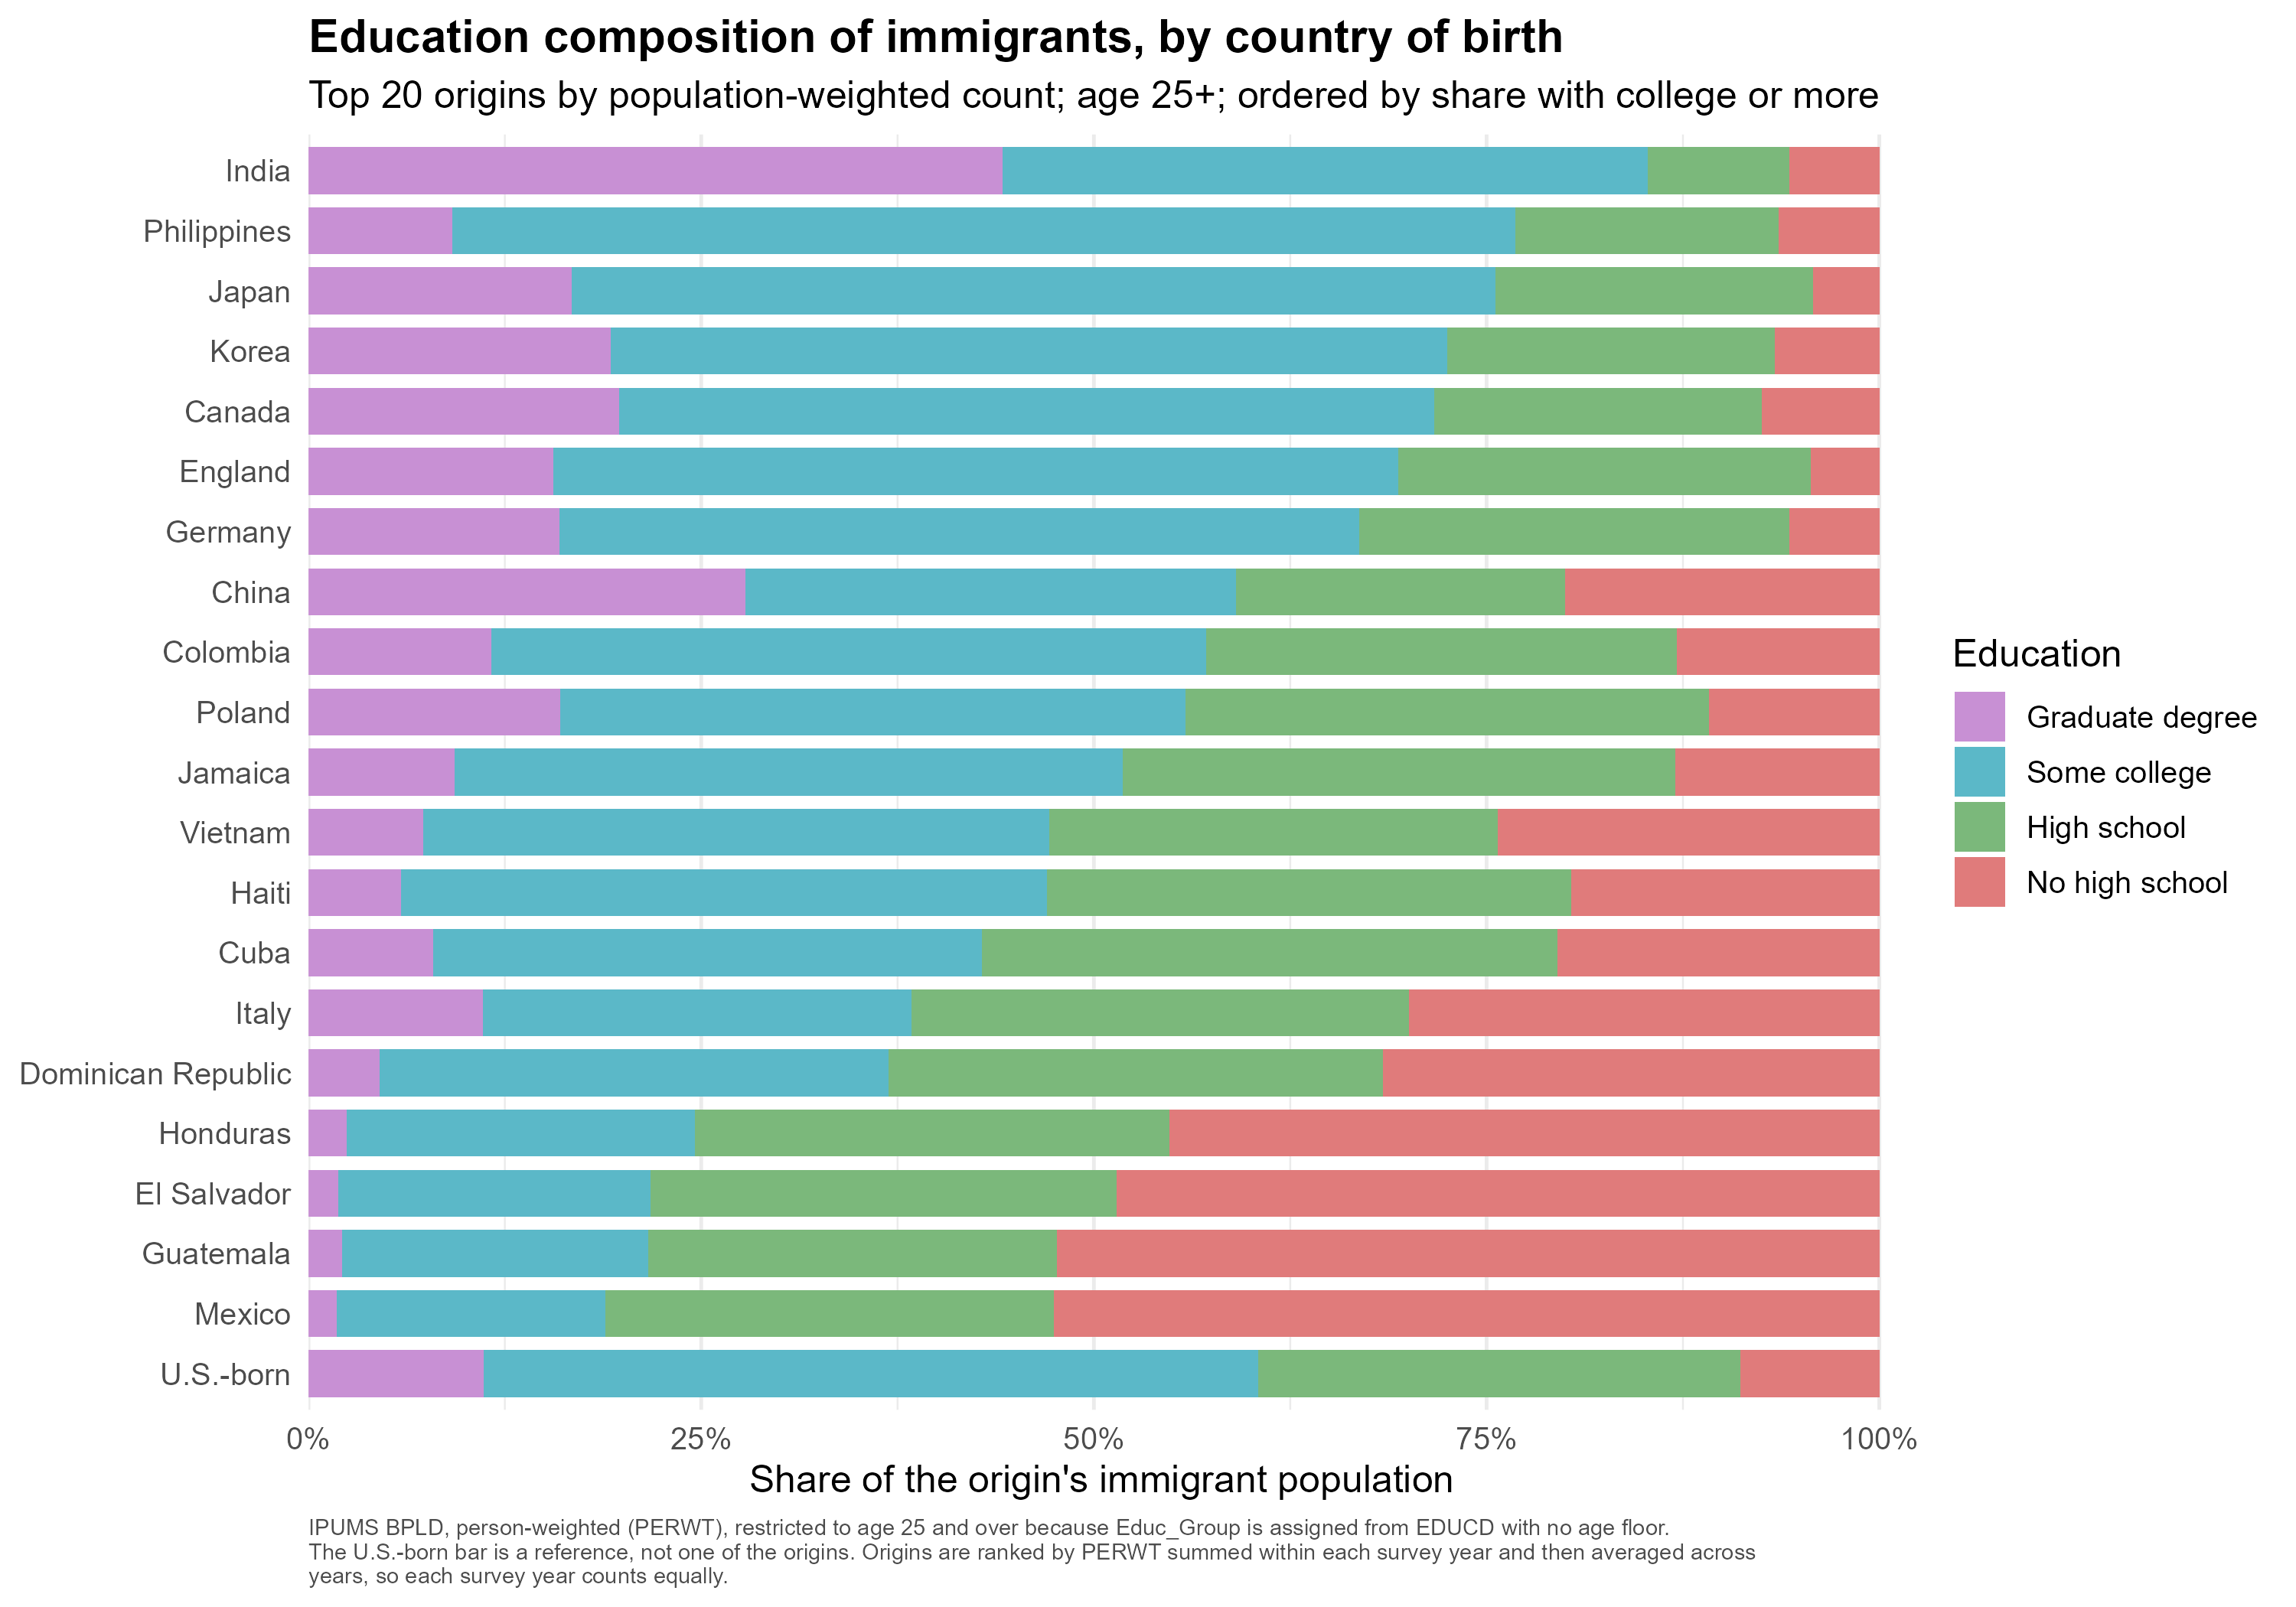
\includegraphics[width=\textwidth]{Educ_By_Origin.png}
    \caption{Education composition of immigrants by country of birth, ages 25
    and older. Origins are the largest by population-weighted count of
    arrivals; bars give each origin's own education distribution, so they are
    within-origin shares and are unaffected by the sampling design's
    overrepresentation of the foreign-born. The U.S.-born bar is drawn as a
    reference and is not one of the origins. The ordering of origin groups
    spans a wider range than the distance between any single origin and the
    U.S.-born distribution, which is the basis for disaggregating immigrants
    by origin rather than treating them as one category. The five origins
    reported numerically in Table~\ref{tab:demographic_summary} are a subset
    of those shown here.}
    \label{fig:educ_by_origin}
\end{figure}

The two ingredients of the instrument constructed below are geographic in different senses, and both bear description before they are put to work. National arrival flows by country of birth supply the shocks; the 1990 distribution of already-settled co-nationals across metropolitan areas supplies the shares. Figure~\ref{fig:origin_world} shows the first of these, giving each country's share of all U.S. arrivals in 1990, 2005 and 2019. What moves across those panels is the weight carried by a largely fixed set of origins rather than the set itself: 162 of the 172 origins in the figure send arrivals in all three years, while Mexico's share of all arrivals falls from 32.7 to 12.4 per cent and India's and China's rise by 5.7 and 4.2 percentage points, with 34.5 percentage points of share reallocated across origins in total. That combination is what the design requires, since an origin absent from the 1990 base carries no share and therefore no weight, however much it later sends. Figure~\ref{fig:dest_americas} shows the destination side for the Americas, the largest sending region; the remaining four regions are reported in Appendix~\ref{sec:immigration_appendix_maps}. Each map uses two channels: hue gives the five-year wave in which that metropolitan area drew its largest share of the region's U.S. arrivals, and opacity gives how many arrivals it received in total. Timing and magnitude are therefore separable by eye, which matters because the two need not coincide -- a metropolitan area can take a late peak on a small flow, or an early one on a large flow.

Read that way, the five regions do not arrive on the same schedule. The Americas are the bimodal case: 83 metropolitan areas peak in 2000--2004 and 96 in 2015--2019, with the two intervening waves accounting for materially fewer. Europe and Australia are the only sending region whose most common peak is the earliest wave, with 72 of 224 metropolitan areas drawing their largest European share in 2000--2004, while the Middle East and Africa tilt decisively late -- 87 of 126 and 90 of 159 metropolitan areas respectively peak in the two most recent waves -- and Asia sits between the two patterns. These maps are descriptive and are drawn across all metropolitan areas clearing a minimum-arrival threshold rather than across the 175 metropolitan areas of the estimation sample; none of the identifying variation used below is read off them.

\begin{figure}[htbp]
    \centering
    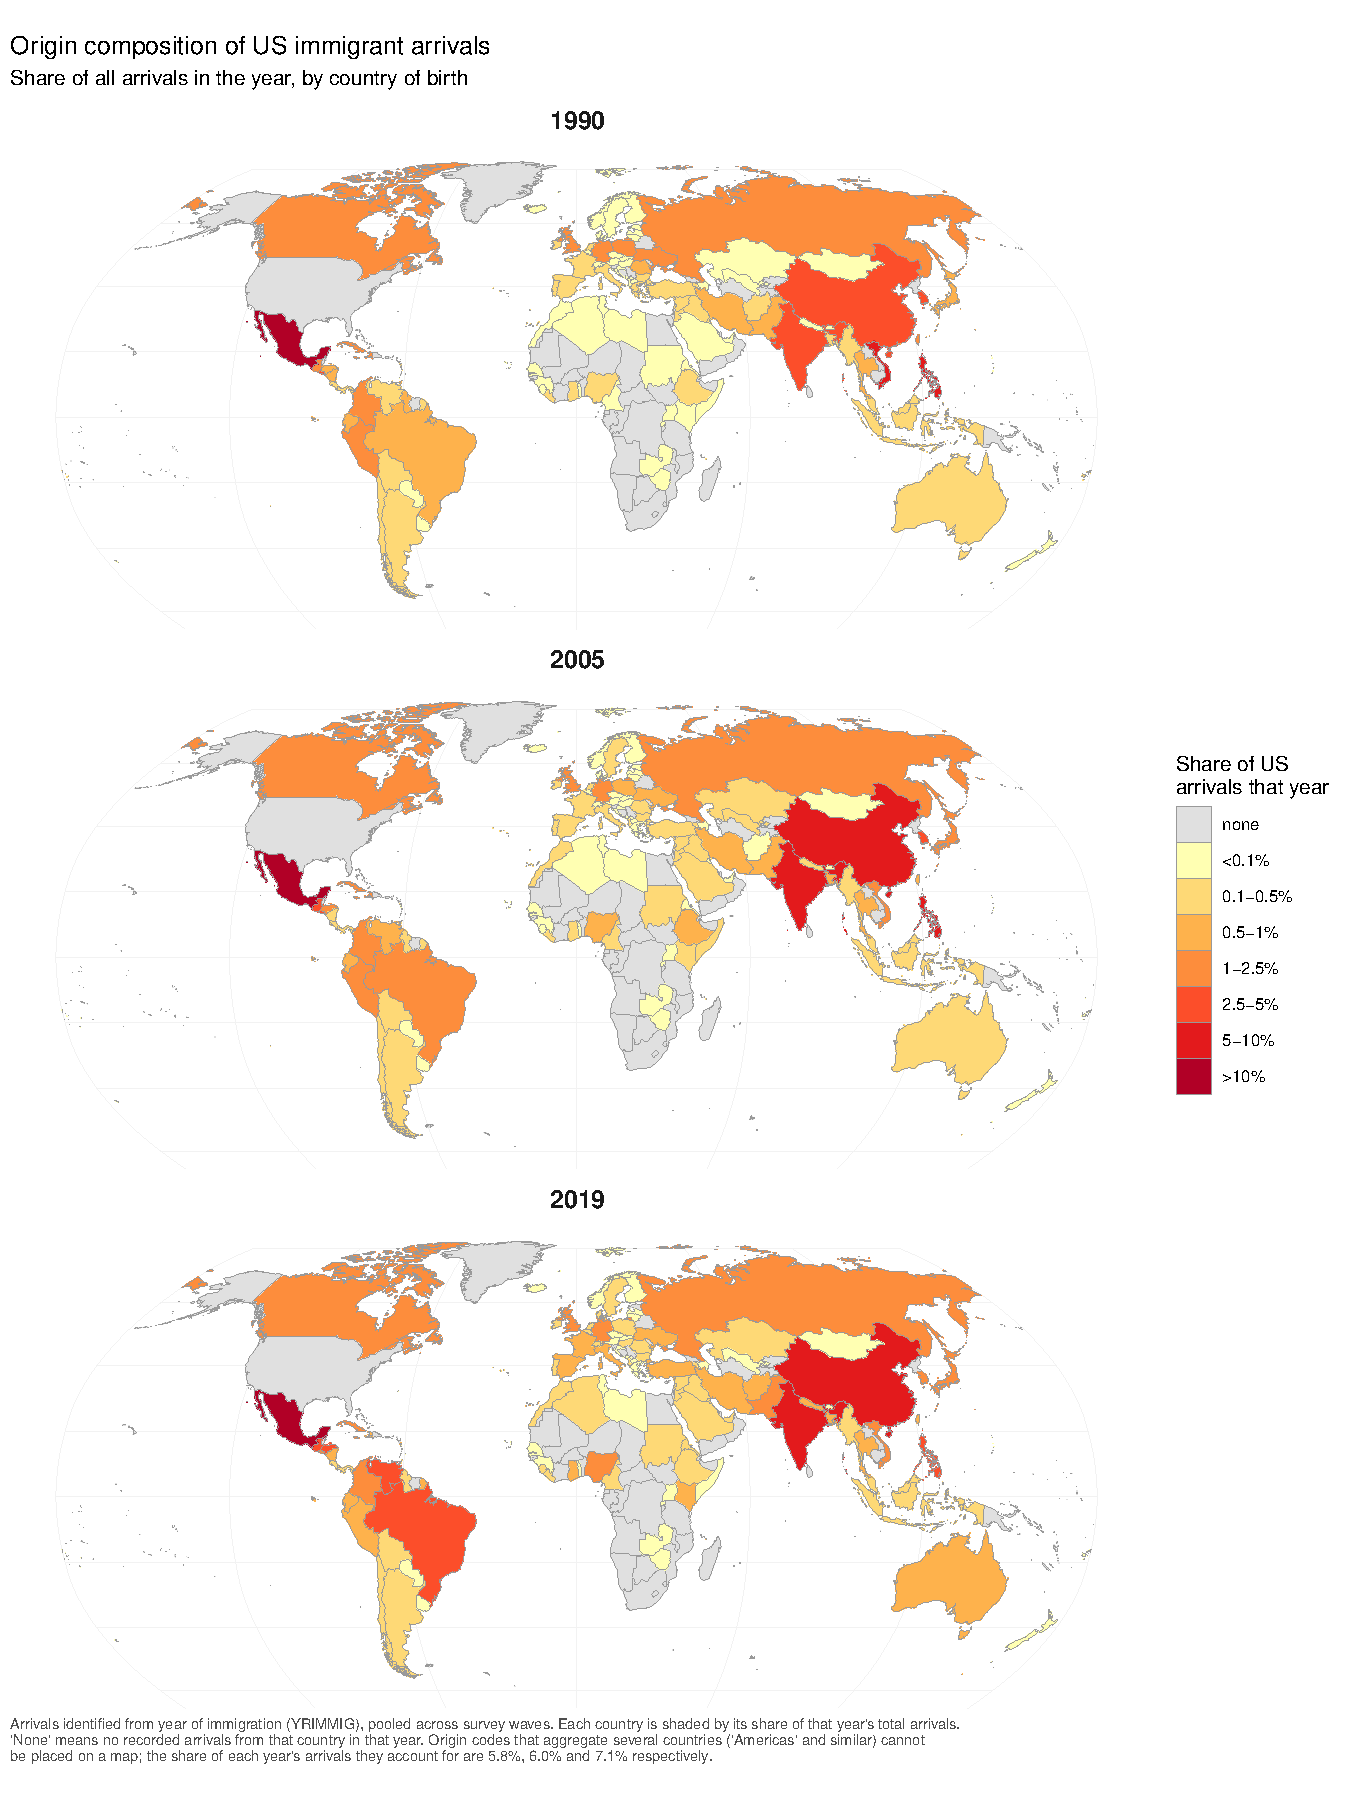
\includegraphics[height=0.85\textheight,keepaspectratio]{fig_origin_world.pdf}
    \caption{Origin composition of U.S. immigrant arrivals in 1990, 2005 and
    2019. Each country is shaded by its share of all arrivals reported in that
    year, identified from year of immigration (\texttt{YRIMMIG}) pooled across
    every survey wave that observes the arrival. 2019 is used in place of a
    later year to avoid the 2020--2021 collapse in recorded arrivals. Countries
    that sent no recorded arrivals in a given year are shaded as such rather
    than left blank, so an absence is distinguishable from a country the
    underlying boundary file does not match; the share of arrivals that could
    not be matched to a mapped country is reported in each panel label.}
    \label{fig:origin_world}
\end{figure}

\begin{figure}[htbp]
\centering
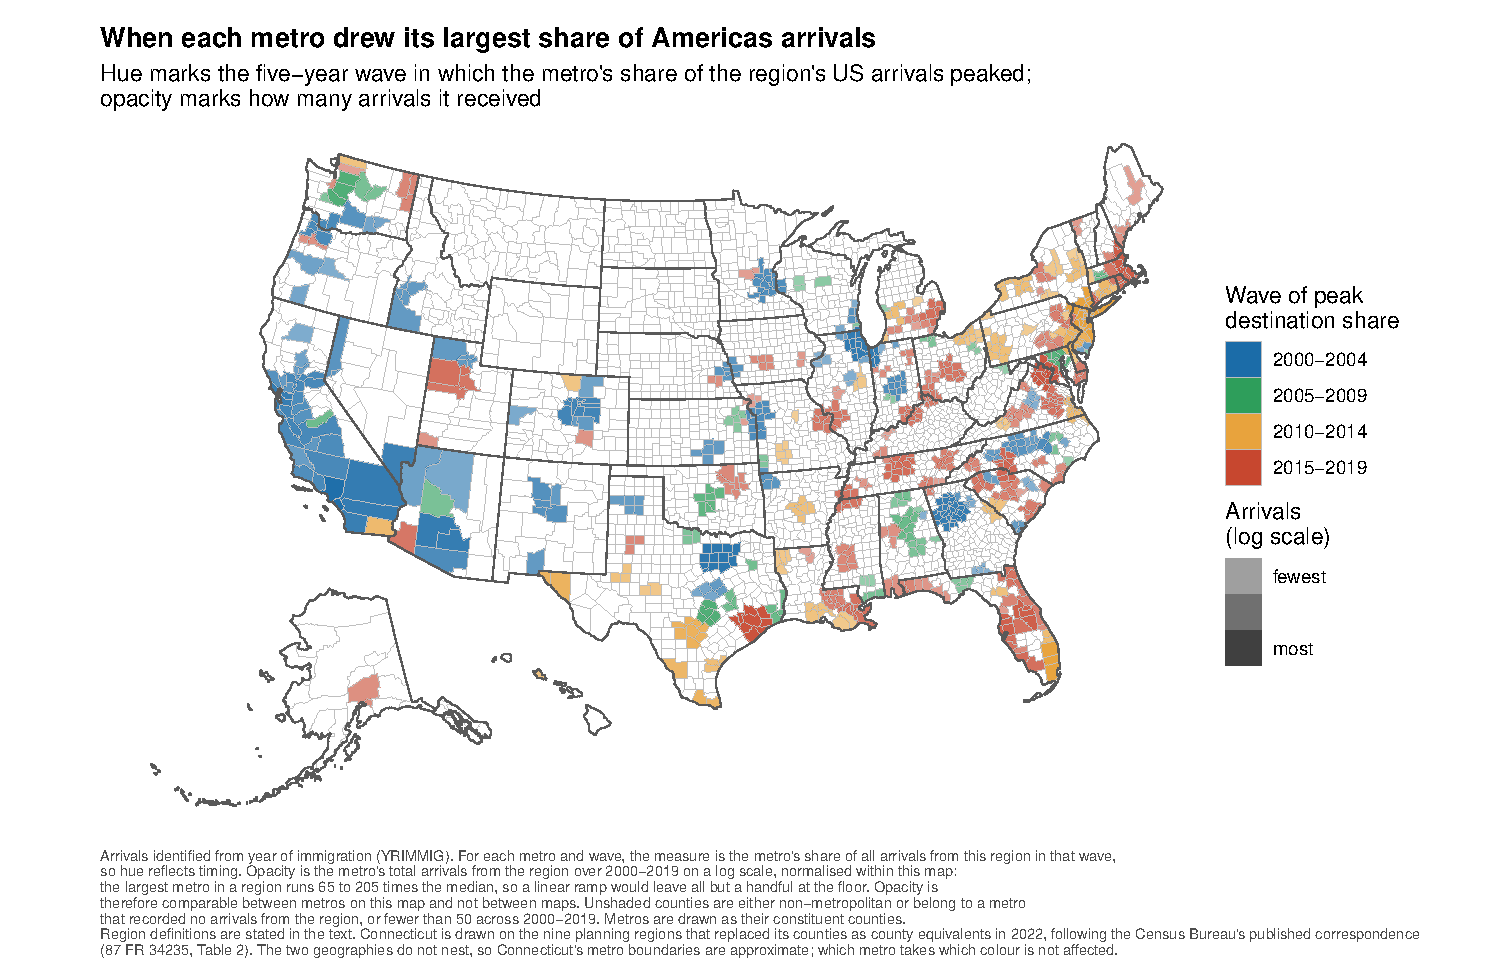
\includegraphics[width=\textwidth]{fig_destination_americas.pdf}
\caption{Metropolitan destinations of arrivals from the Americas, by peak
five-year wave. Hue marks the wave in which each metropolitan area drew its
largest share of all U.S. arrivals from the Americas, so hue reflects
timing. Opacity marks the metropolitan area's total arrivals from the region
over 2000--2019, on a log scale normalised within each map: the largest
metropolitan area in a region receives between 65 and 205 times the median,
so a linear ramp would leave all but a handful at the floor. Opacity is
therefore comparable between metropolitan areas within a map and not between
maps. Unshaded counties are non-metropolitan, or belong to a metropolitan
area recording too few arrivals from the Americas over 2000--2019 to assign a
peak.
Metropolitan areas are drawn as their constituent counties; Connecticut is
drawn on the nine planning regions that replaced its counties as county
equivalents in 2022, following the Census Bureau's published correspondence
(87 FR 34235, Table 2). The two Connecticut geographies do not nest, so its
metropolitan boundaries are approximate, though which metropolitan area takes
which colour is unaffected. Puerto Rico is omitted. The corresponding maps
for the other four sending regions are reported in
Appendix~\ref{sec:immigration_appendix}.}
\label{fig:dest_americas}
\end{figure}

The exposure measure is a count of arrivals and carries no natural unit, so effects are reported throughout against a one-standard-deviation increase rather than against a one-unit increase. Table~\ref{tab:exposure_distribution} gives the distribution that scaling refers to, and three features of it bear on how the estimates below should be read. The first is skew: the median identifying observation carries a predicted inflow of 451 against a mean of 3,084 and a ninetieth percentile of 8,696, so the standard deviation of 6,545 is set by a long right tail of large gateway metropolitan areas rather than by anything typical. The second is that treatment is defined jointly by place and cohort -- 5,775 distinct values across 175 metropolitan areas and 33 birth cohorts -- so exposure separates individuals enumerated in the same city in the same year who passed through adolescence at different times. The third is where that variation sits. Metropolitan-area means account for 72.3 per cent of the instrument's variance and birth-cohort means for 5.1 per cent; because the specifications below absorb metropolitan-area and survey-year effects, the between-city component is removed before estimation, and the spread that survives it -- 3,427, a little over half the raw figure -- is what identifies the coefficients. That so little of the total rests on the cohort margin is worth noting on a separate count: the component moving identically across every city within a cohort is not what supplies the instrument its variation.

\input{table_exposure_distribution}

Two data limitations warrant explicit note. First, no data exist for 2001--2005: the panel jumps directly from the 2000 decennial census to the 2006 ACS, so any figure or table constructed from year-level aggregates should be read as having no observations in that four-year window rather than as showing a smooth interpolation across it. Second, parental education records are missing for the majority of the estimation sample: \texttt{Mom\_Educ} is unavailable for 68.6 percent of observations and \texttt{Dad\_Educ} for 74.9 percent (Table~\ref{tab:parent_educ_missing}), both coded as an explicit ``Missing'' category rather than imputed or dropped. This reflects a structural feature of the underlying IPUMS variables rather than random nonresponse: \texttt{EDUC\_MOM} and \texttt{EDUC\_POP} are constructed by linking each individual to a coresident parent's record, and are populated only when that parent lives in the same household at the time of the survey -- a condition satisfied for most children and young adults but not for the majority of the adult population, who have left the parental home by the time they are observed. Both variables are retained as controls throughout the empirical analysis, but their explanatory content is effectively limited to the minority of the sample still coresiding with a parent.


% =============================================================================
\section{Identification Strategy}
\label{sec:immigration_id}
% =============================================================================

A causal estimate of the effect of immigrant exposure on U.S.-born educational attainment cannot be recovered from a direct regression of educational outcomes on immigrant inflows, because the contemporaneous immigrant share of a metropolitan area is not independent of the very economic conditions that also shape U.S.-born human capital investment. Metropolitan areas experiencing positive labor demand shocks attract immigrants and simultaneously raise the returns to schooling for U.S.-born residents through channels entirely unrelated to immigrant exposure itself; conversely, U.S.-born individuals with strong unobserved determinants of educational attainment may selectively reside in, or move to, metropolitan areas that also happen to receive large immigrant inflows. Either channel would bias a direct regression of educational attainment on the actual immigrant inflow, in a direction that is not, in general, signable. Following \citet{card2001immigrant} and \citet{altonjicard1991effects}, this paper addresses this endogeneity with a shift-share instrument: a predicted, rather than actual, measure of immigrant inflow constructed from variation that is plausibly unrelated to contemporaneous local demand conditions.

The instrument combines two ingredients. The first is the 1990 distribution of established immigrant communities: for each origin country $k$, $s_{m,k}$ denotes the share of all immigrants from origin $k$ residing in MSA $m$ in 1990, out of all immigrants from origin $k$ residing in any of the 175 stable MSAs in 1990. The base year is a choice rather than a data constraint: metropolitan detail runs back well before 1990, and a 1980 base would admit ten further birth cohorts. It is rejected on relevance. Shares measured before 1965 describe the settlement of a different population, the Immigration and Nationality Act of that year having shifted origin composition from predominantly European to predominantly Asian and Latin American, so a 1950 or 1960 share vector carries near-zero weight for the origins that supply most of the identifying variation reported below; 1970 falls too soon after the Act for the new patterns to have consolidated geographically; and 1980, the genuine alternative, predicts allocation over the sample period less well than 1990 does, which matters because a ten-year exposure window requires the shares to stay close enough to the exposure period to retain a first stage. The 1990 base also precedes the formative-years window of every individual in the estimation sample, so $s_{m,k}$ cannot itself respond to the labor market conditions realized over that window. The second ingredient is $\Delta_{k,t}$, the national-level inflow of immigrants from origin $k$ arriving in year $t$. Both the decennial census and the ACS ask immigrants what year they arrived in the United States (\texttt{YRIMMIG}), which permits $\Delta_{k,t}$ to be reconstructed for every year from 1910 to 2023 rather than only for the years in which the underlying survey was fielded. $\Delta_{k,t}$ is the pooled count of respondents reporting arrival from origin $k$ in year $t$, taken across all survey waves that observe them and left unnormalized. Because the shift-share instrument and the endogenous variable are constructed from this same series and evaluated over the same window, any factor common to an arrival year -- including the number of survey waves in which that year's arrivals remain observable -- enters the predicted and realized inflows alike, and the exposure measure is a comparison between the two rather than a statement about the level of either.

Combining the shares and shocks yields the predicted immigrant inflow to MSA $m$ in year $t$, $\text{predicted\_inflow}_{m,t} = \sum_k s_{m,k}\,\Delta_{k,t}$ -- the shift-share, or Bartik, instrument in its standard form: MSAs with an established 1990 population from origin countries that subsequently send large numbers of new immigrants nationally are predicted to receive large inflows, independent of any labor market conditions specific to MSA $m$ after 1990. Because the outcome of interest is measured at the individual level and the formative years relevant to educational investment are fixed by birth year rather than by calendar year, this MSA-year instrument is converted into an individual-level exposure measure. For each U.S.-born individual $i$ residing in MSA $m$, the instrument is $z_i = \frac{1}{|W_i|}\sum_{t \in W_i} \text{predicted\_inflow}_{m,t}$, where $W_i$ is the set of calendar years in which individual $i$ was between the ages of 15 and 25. This captures the predicted immigrant inflow to an individual's own metropolitan area across the decade in which educational investment decisions are typically made, rather than the inflow at any single point in time. The window is bounded below by 1990, the base year of the shares, and above by the last year for which arrival data are available, so $|W_i|$ is eleven for most individuals and fewer for those whose window is truncated at either end.

The endogenous regressor is constructed by applying the identical operation to the realized series: $x_i = \frac{1}{|W_i|}\sum_{t \in W_i} \text{actual\_inflow}_{m,t}$, the actual immigrant inflow to the individual's metropolitan area averaged over \emph{the same} window $W_i$. This correspondence is the substantive content of the design rather than a matter of bookkeeping. Educational investment responds to the immigrant presence an individual encounters while deciding how much schooling to acquire, not to the immigrant presence in the year a survey happens to enumerate them, and for most of the sample those are separated by years or decades. Instrumenting a contemporaneous regressor with a windowed instrument would ask whether predicted exposure during adolescence predicts realized inflows at the moment of enumeration, which is a different question with no clear interpretation. Because $z_i$ and $x_i$ are the predicted and realized versions of one quantity measured over one window, the first stage has a direct reading: the degree to which historical settlement patterns predict the immigrant inflows an individual actually experienced during their formative years.

Both series are indexed by \emph{arrival} year: the subscript $t$ records the year in which immigrants entered the country, recovered from \texttt{YRIMMIG}. The estimation sample, by contrast, is indexed by \emph{survey} year, since U.S.-born respondents have no arrival year and are observed in the wave that enumerates them. The windowing above is what connects the two indices, evaluating an arrival-year-indexed series at the calendar years spanning each individual's ages 15 through 25.

Exposure is zero by construction for individuals whose ages-15--25 window opens before 1990, since no predicted inflow exists for those years. These individuals are flagged with an indicator, $\text{exposure\_missing}$, included as a control in every specification. They are retained rather than dropped -- they contribute to the estimation of the controls and the fixed effects -- but they supply no variation in the instrument, so identification rests on the remainder. Section~\ref{sec:immigration_robustness} reports the specification restricted to that identifying subsample.

Exposure is a deterministic function of metropolitan area and birth year: two U.S.-born individuals living in the same metropolitan area and born in the same year face the same window, the same predicted inflows, and are assigned identical values of $z_i$ and $x_i$. The treatment is therefore defined at the metropolitan-area by birth-cohort level, and across 175 metropolitan areas and the 33 birth cohorts with non-zero exposure it takes 5{,}775 distinct values.

Three consequences follow. The first concerns what is being estimated: the parameter is the effect of belonging to a higher-exposure metropolitan-area-by-cohort cell, so any individual-level mechanism is an interpretation placed on a cell-level result rather than something the design identifies directly. The second concerns where precision comes from. Standard errors are clustered on metropolitan area, which is above the level at which treatment is assigned, so precision derives from variation across the 175 clusters rather than from the number of individuals within them; what the 8,537,597 individual records contribute is national coverage -- 45 states over three decades -- and the covariate detail the outcome equation requires. The third is the most consequential for specification: metropolitan-area, survey-year and age fixed effects cannot be included together. Birth cohort is the difference between survey year and age, so a model containing all three absorbs the dimension along which treatment is assigned and leaves no variation in exposure to identify a coefficient from.

The cost of defining treatment at this level is the counterpart of its identifying power. Any influence on educational attainment that varies at the metropolitan-area by birth-cohort level and correlates with immigrant inflows cannot be separated from the effect of exposure. Metropolitan-area fixed effects absorb whatever is fixed about a city across cohorts, and survey-year fixed effects absorb whatever is common to the nation in a year, but a shock specific to one city's cohorts -- a local change in school funding or labour demand that happened to track immigrant arrivals -- is not separable from the exposure measure. \citet{card2001immigrant} confronts a structurally identical problem. His wage and employment equations include both occupation and city fixed effects, which absorb anything common to an occupation nationally or to a city across occupations; what remains in the error term, as he notes, are occupation-specific local productivity shocks, and these bias the estimated coefficient upward whenever a local shock raises wages and draws workers into the occupation. The disturbance that defeats his fixed effects sits at the interaction of the two dimensions whose margins they absorb, exactly as a metropolitan-area-by-cohort shock sits at the interaction here. His remedy is the instrument this paper also uses -- historical settlement patterns interacted with national arrival flows -- selected because it is correlated with local supply but plausibly not with the interaction-level shock. The present design substitutes birth cohort for occupation as the second dimension; the logic, and the residual vulnerability, are the same.

Identification requires that the 1990 origin-country shares $s_{m,k}$ be uncorrelated with future MSA-level shocks to the returns to education, conditional on MSA and year fixed effects -- the same assumption underlying \citet{card2001immigrant}'s use of this design to study native outflows. Formally, this rules out any channel by which an MSA's historical immigrant settlement composition predicts subsequent shocks to local labor demand or school quality except through the immigrant inflows the instrument is designed to capture. This assumption has recently become the subject of substantial methodological scrutiny in its own right, and the remainder of this section subjects the design to four separate diagnostics addressing that literature directly.

Instrument relevance is not a first-order concern for this design. The first stage, reported in Table~\ref{tab:education_main}, is $0.647$ with a metropolitan-area-clustered standard error of $0.105$, a $t$-statistic of $6.14$ on 175 clusters. Because inference here is governed by the cluster count rather than by the number of individual observations, the conventional $F$-statistic threshold of 10 \citep{stock2002testing} is reported against a sample whose effective size is the cluster count, and the relevant comparison is the clustered $t$-statistic rather than a homoskedastic $F$ computed over millions of rows, which would be inflated by replication of a regressor that varies only across metropolitan areas and cohorts. The remaining concerns raised in the shift-share literature are accordingly ones of exogeneity and inference rather than relevance, and the four most salient are taken in turn.

 \citet{goldsmith2020bartik} show that a shift-share estimator is numerically equivalent to a GMM estimator using the underlying shares as instruments, each weighted by what they term a Rotemberg weight. Under this view identification does not rest on the instrument as a whole but on the exogeneity of whichever origin shares carry the most weight: if one or two groups dominate, validity turns narrowly on those groups' shares being uncorrelated with local shocks to educational attainment. Table~\ref{tab:rotemberg} reports the decomposition. Two features of it bear on the credibility of the design. The first is how few origins contribute at all: of the 230 origin regions in the inflow series, 148 carry non-zero weight. The 82 that do not are, with four exceptions, observed in the 1990 base and therefore carry a non-zero share in at least one metropolitan area; what they lack is arrivals in any year falling inside an individual's exposure window, so it is the shock rather than the share that reduces their contribution to zero. Only four origins are absent from the 1990 base altogether. Of the 148 that do contribute, 146 carry positive weight, and the two negative weights are negligible against a total of one. The second is the degree of concentration among those that do contribute. Mexico, the largest, accounts for 18.9 per cent of identifying weight; the five largest account for 42.2 per cent and the ten largest for 56.6 per cent. That is concentrated, but it is not domination by a single share, and every one of the ten highest-weighted origins returns a just-identified estimate of the same sign, ranging from $6.9 \times 10^{-6}$ to $1.5 \times 10^{-5}$ around an aggregate of $1.1 \times 10^{-5}$.

\input{table_rotemberg}

Concentration alone is not a verdict, since a concentrated design can still be sound if the dominant shares are exogenous and a dispersed one unsound if they are not. The sharper test is whether the estimate depends on them, and Table~\ref{tab:rotemberg_sensitivity} reports it directly: removing Mexico alone moves the estimate by $-3.3$ per cent, and removing the ten largest origins -- 56.6 per cent of the identifying weight -- moves it by $-4.5$ per cent. The estimate is not an artefact of any one origin's settlement pattern, which is the specific fragility the decomposition is designed to expose. The changes are not monotone in the number of origins removed; with half the weight gone the estimate rests on a different and much smaller set of shares, and the small non-monotonicities across those columns should not be read as structure.

\input{table_rotemberg_sensitivity}

A second concern, raised by \citet{adao2019shift}, is that conventional standard errors in shift-share designs can be understated, because the underlying shocks induce correlation across units with similar exposure shares rather than merely across units that are geographically close -- a form of dependence that simple geographic clustering will not detect. The design is tested against this concern in two ways, reported in Table~\ref{tab:adao_placebo}. The first is a set of placebo outcomes determined at birth and therefore incapable of responding to immigration during adolescence: indicators for Black, Aboriginal and Asian identity. Black identity shows no relationship with the instrument ($t = 0.53$, $p = 0.60$ under metropolitan-area clustering), and Aboriginal identity none ($t = -0.05$, $p = 0.96$); expressed on the scale of the educational estimate they amount to 4.3 and 0.02 per cent of it respectively, which is the comparison that matters on a sample this size. Asian identity does not pass, at $t = 2.81$ ($p = 0.005$) and 14.3 per cent of the reference effect. It reflects the concentration of Asian population shares in the metropolitan areas where Asian immigration has historically settled, and its significance strengthens rather than weakens under state clustering ($t = 3.60$), which is the opposite of what a failure of inference would produce. Adding an Asian indicator to the control set moves the main estimate by roughly one tenth of one per cent, reported in column (3) of Table~\ref{tab:education_main}, which locates the problem in composition rather than in a channel through which the instrument acts on attainment.

\input{table_adao_placebo}

The second test speaks to the \citet{adao2019shift} mechanism directly. Table~\ref{tab:education_main} reports both metropolitan-area-clustered and state-clustered standard errors for every coefficient, so their ratio can be formed where it is wanted; on the headline two-stage least squares estimate it is $0.880$. State clustering produces the \emph{smaller} standard error, where unmodelled correlation across similarly exposed units would produce the larger one. There is no evidence of the dependence \citet{adao2019shift} describe, which is not the same as establishing its absence. Coarsening the cluster definition also cuts the number of clusters from 175 to 45, and cluster-robust variance is more downward-biased the fewer clusters there are, so part of any reduction is attributable to the cluster count rather than to the correlation structure. A ratio above one would have been the informative result.

\citet{borusyak2022quasi} relocate the identifying assumption from the shares to the shocks: what consistency and valid inference require is many quasi-randomly assigned shocks rather than many geographic units. A design whose shocks arrived only with the decennial census would be weak on that criterion however many individuals it observed, and the shocks here are annual, the inflow series being reconstructed from arrival year rather than survey year. How many of those annual shocks are independent is not something this design can establish, since national inflows are serially correlated within origin, so what answers the critique is not a count. It is the placebo already reported in Table~\ref{tab:adao_placebo}, and the sum-of-shares control that an instrument built from incomplete shares requires, reported next.

One further requirement of their framework applies where the exposure shares do not sum to one within a unit, as the national-share formulation used here does not: the instrument is then a weighted sum rather than a weighted average of the national inflows, and a metropolitan area holding a larger total share receives a systematically larger instrument value even under randomly assigned inflows. Table~\ref{tab:bhj_incomplete_shares} reports the control \citet{borusyak2022quasi} prescribe for this case, the sum of shares interacted with the effects for the period of the inflow. It absorbs rather more than half of the instrument's identifying variation, leaving a standard deviation of $1{,}618$ against $3{,}427$, and the estimate holds: the reduced form moves by $1.2$ standard errors and the two-stage estimate by $0.7$, both remain significant, and the first stage is estimated as precisely as in the baseline. The first-stage coefficient does fall by half, which locates much of the instrument's power to predict realized local inflows in the scale and timing of a metropolitan area's total immigration rather than in its origin composition.

\input{table_bhj_incomplete_shares}

A fourth concern, raised by \citet{jaeger2018shift}, is structural rather than statistical. Because immigrant settlement is persistent -- new arrivals from an origin tend to settle where earlier arrivals from that origin already live -- and because national inflows are themselves serially correlated, a shift-share instrument built from a base-year share and a contemporaneous shock can conflate the immediate effect of current immigration with the accumulated response to decades of prior immigration to which a local labour market has already partly adjusted. Their proposed remedy is to instrument with contemporaneous and lagged shift-shares jointly, so that the two horizons can be separated.

Three features of the present design bear on this. The first is the base year. The shares are fixed at 1990 and never updated, so the settlement patterns it uses predate all but the earliest of the arrivals it is used to predict -- the self-prediction that motivates the \citet{jaeger2018shift} critique is at its weakest with a base this distant from most of the sample. The second is that the conflation they describe is aimed at a different kind of estimate. Their concern is that a short-run labour market response is contaminated by the accumulated response to earlier immigration; here both sides of the design are cumulative by construction, the instrument being an eleven-year average of predicted inflows and the outcome a stock of completed schooling rather than a flow. An attainment stock measured over a decade-long window is a poor target for a critique about contemporaneous impact effects. What persistence does threaten in this design is narrower, and is taken up next.

The third feature is a genuine cost rather than a response, and it follows from the same persistence \citet{jaeger2018shift} identify. Because settlement persists and the exposure window spans eleven years, individuals born in adjacent years share ten of those eleven years of predicted inflow, so exposure is strongly autocorrelated across the cohort dimension and two cohorts must be a decade apart before their windows are disjoint. The independent variation in the instrument is accordingly a good deal smaller than the number of metropolitan-area-by-cohort cells suggests. This is the limitation declared at the outset of this section rather than a separate finding: treatment is defined at the metropolitan-area by birth-cohort level, that dimension is serially correlated by construction, and influences varying along it cannot be separated from the effect of exposure.

\section{Results}
\label{sec:immigration_results}

Table~\ref{tab:education_main} reports the main estimates. All specifications are linear probability models estimated on the full sample of 8,537,597 U.S.-born observations in the 175 stable MSAs, with year and MSA fixed effects, the individual-level controls described in Section~\ref{sec:immigration_data}, and standard errors clustered on MSA. No age restriction is imposed; the ages 25 and older convention used in the descriptive tables of Section~\ref{sec:immigration_data} applies to those tables alone, so the sample sizes reported there and here are not comparable.

\input{table_education_main}

The first stage is positive and strong: a one-unit increase in predicted inflow over an individual's ages 15--25 window is associated with a $0.647$ increase in the actual inflow measured over that same window ($t = 6.14$). That the instrument and the endogenous variable are evaluated over the identical window is not incidental and matters for interpretation: the endogenous variable is the average actual inflow across ages 15 through 25, not the inflow in the survey year, so the first stage asks whether predicted and realized exposure move together over the same decade of an individual's life rather than at an arbitrary later date.

Both education margins respond. On the high-school margin -- completing high school or more, against failing to complete high school -- the reduced-form coefficient is $7.25 \times 10^{-6}$ with a clustered standard error of $7.34 \times 10^{-7}$, and the two-stage least squares estimate is $1.12 \times 10^{-5}$. On the college margin -- completing some college or above, against all lower attainment -- the reduced form is $5.31 \times 10^{-6}$ and the two-stage least squares estimate is $8.20 \times 10^{-6}$. Both are significant at conventional levels under MSA clustering; the shock-randomization placebo of \citet{adao2019shift} in Table~\ref{tab:adao_placebo} is the inference test this design ultimately rests on.

Raw coefficients of this order are not directly interpretable, because they are expressed per unit of inflow. The final column rescales the reduced form to a one-standard-deviation increase in exposure among the observations that identify it: $4.74$ percentage points on the high-school margin and $3.47$ percentage points on the college margin. The standard deviation in question is that of the metropolitan-area-by-cohort exposure measure across identifying observations, so the figure should be read as the difference between cells one standard deviation apart in exposure rather than as a change experienced by any individual. The ordering is itself informative. A design in which immigrant exposure operated principally by displacing U.S.-born students from constrained educational institutions would be expected to produce its largest effects where capacity binds most tightly; finding a positive response at both margins, and the larger of the two at the point of high school completion, is more consistent with the human capital investment channel implied by the task-reallocation literature \citep{peri2009task, mchenry2015immigration} than with a crowding-out account.

The binary outcome collapses four attainment categories into one threshold, which raises the question of whether it conceals movement among the higher levels. Table~\ref{tab:multinomial} answers it by estimating the same specification with the four-category outcome on a random draw of 100,000 observations, with the binary model re-estimated on that same draw, and converting both to average marginal effects, which are comparable where raw multinomial coefficients are not. The figures below are therefore on the draw rather than the full sample. The decomposition reproduces the binary estimate almost exactly: the implied effect on completing high school or above is the negative of the marginal effect on the no-high-school category, and the two agree to within one per cent (5.48 against 5.43 percentage points per standard deviation). The multinomial therefore carries no information about the effect's magnitude that the binary specification does not already carry.

What it adds is a description of where the movement out of no-high-school goes, and the answer is that it goes nowhere in particular. Each completing category's share of the effect tracks its share of the completing population closely; no category absorbs a disproportionate part of the movement and none moves against the others. The redistribution is roughly what a draw from the existing attainment distribution would produce. That is itself the finding: the effect operates on the decision to complete secondary schooling at all, not on the choice among higher levels conditional on completing, and it is the reason the binary specification is sufficient for the rest of the chapter.

Two limits on how far that should be read. The draw is used because the full-sample multinomial is a ten-day computation and the question it answers is settled without it. And the individual category effects are imprecise: the bootstrap behind them is coarse by design, sized for deciding whether the decomposition is informative rather than for inference on any one category. The proportionality is the claim; the individual magnitudes are not.

\input{table_multinomial}

The third row of Table~\ref{tab:education_main} adds indicators for Asian and Aboriginal identity to the control set, in response to the placebo diagnostic in Table~\ref{tab:adao_placebo}. The estimate moves by roughly one tenth of one per cent, which establishes that the Asian placebo failure reflects the composition of gateway metropolitan areas rather than a channel through which the instrument acts on educational attainment.

A $4.74$ percentage point increase in high school completion per standard deviation of immigrant exposure is reported per standard deviation because the exposure measure is a count of arrivals and carries no natural unit of its own, which leaves it not directly comparable to \citet{hunt2017impact}, whose coefficient is per percentage point of the immigrant population share. The two can be placed on a common footing using a scaling Hunt supplies: one percentage point of her immigrant share is $0.13$ of that variable's standard deviation, so her preferred estimate of $0.34$ percentage points -- $0.3$ in the abstract's rounding -- is approximately $2.6$ percentage points per standard deviation of the immigrant variable, against $4.74$ here. Standardising aligns the scales without making the regressors the same object: hers is a stock share and the measure used here is a flow of arrivals. The remaining difference is a factor of roughly two rather than the order of magnitude the raw coefficients suggest, and the most likely explanation is structural rather than causal. Because the exposure window is fixed by birth year, the individuals carrying the largest exposure values are mechanically the youngest in the sample, and the youngest are also those most likely to be recorded as not having completed a given level of schooling simply because they have not yet finished it. Section~\ref{sec:immigration_robustness} quantifies this directly.

The design treats the metropolitan area as the unit of exposure, so a U.S.-born individual who grows up in a high-inflow metro is taken to have encountered those inflows. If instead U.S.-born residents left in response to immigrant arrivals, metropolitan composition would respond endogenously to the instrument and the exposure measure would be contaminated by selective departure. \citet{card2001immigrant} puts the same question to his own design and finds that immigrant inflows do not induce compensating outflows.

\input{table_migration_iv}

Table~\ref{tab:migration_iv} reports the replication. The outcome is an indicator for having changed metropolitan area in the past year, and inflow is measured contemporaneously with the survey rather than over the formative-years window: the question is whether individuals respond to current immigration, so the windowed construction used for educational attainment does not apply. Two specifications are reported for each group, differing in sample and in instrument, and none of the six estimates is distinguishable from zero. The levels specification returns $p$-values of 0.12, 0.75 and 0.42 for all U.S.-born respondents, men and women respectively; the differenced specification returns 0.30, 0.16 and 0.73. Against a baseline annual inter-metropolitan move rate of 16.5 per cent, the design has ample scope to detect a mobility response and finds none. This replicates \citet{card2001immigrant} on a longer panel and finer geography. Its bearing on the design is that native location does not respond to immigrant arrivals, so the metropolitan area an individual is observed in is not systematically the wrong one as a consequence of the inflows the instrument predicts.

The wage results that follow are a secondary exercise rather than a central claim of this chapter, and are reported because the mechanism proposed for the education result -- that immigrant inflows raise the return to communication-intensive work and so to the schooling that leads to it \citep{peri2009task, mchenry2015immigration} -- carries an implication worth checking: if the return to schooling is what moves, the wage data should show it moving. Mean completed schooling across the occupation groups used below runs from 11.7 years in low-skill labour and service and in operative and craft work to 15.2 among professional and technical workers, so the groups can be ordered on how much schooling they require.

\input{table_wage_iv}

Table~\ref{tab:wage_iv} reports instrumental variables estimates of occupation-specific immigrant inflows on mean hourly wages within metropolitan-area-by-occupation-by-year cells, with metropolitan-area and survey-year fixed effects and standard errors clustered on metropolitan area. The per-standard-deviation column is the comparable one: inflow volume differs by an order of magnitude across occupation groups, so the raw coefficients are measured against different-sized shocks and cannot be read down a column. First stages are strong throughout except among military occupations, with $F$ statistics running from 34 to 997. Five of the seven groups are indistinguishable from zero. Professional and technical workers, the most education-intensive group, gain \$0.53 per hour per standard deviation of own-group inflow, 2.5 per cent of their mean wage; sales workers lose \$0.21, 1.8 per cent, and are the more precisely determined of the two. Among the sex splits the professional and technical gain is larger for men (\$0.77, 3.2 per cent) and not significant for women, the sales loss appears only among men (\$0.29, 2.1 per cent), and the one estimate significant for women but not for men is a loss of \$0.14 in low-skill labour and service.

The absence of a negative effect at the low-skill end of the pooled sample is the result most directly comparable to the existing literature, and it is consistent with \citet{card1990impact} and \citet{card2005new} rather than with a simple competitive-displacement account. It should be read as no detectable effect rather than as a precise zero, and the pooled null is not uniform: the estimate for women in that group is negative and significant. What the two surviving estimates bear on is not where U.S.-born workers end up but why additional schooling would be worth acquiring. The return to the most education-intensive occupation rose, and the return to an alternative requiring less of it fell, which widens the gap that schooling buys. Neither result is a claim about occupational destination, and none is made here: the outcome throughout this chapter is attainment, and the data cannot say which occupations the individuals acquiring that attainment subsequently enter. Nor is a gradient claimed. Managers rank second on completed schooling at 14.3 years and return an estimate indistinguishable from zero, so the contrast is between the top of the education ordering and a mid-table alternative rather than a monotone pattern across it, and it rests on one significant estimate in each direction out of seven. Two limitations qualify the exercise. Cell headcounts are uneven, with a median of 13 to 54 respondents per cell in the pooled columns but 4 to 28 in the sex splits, so the pooled column carries more weight than the disaggregated ones. And military occupations are not identified: the first stage returns an $F$ of 4.6 against 34 or above everywhere else, military pay is set by federal scale rather than by local labour markets, non-citizens are largely barred from service, and the group appears in 1,014 cells with a median of one respondent per cell. The estimates in that row -- including an implausible gain of \$10.23 per hour among women, on 262 cells across 56 metropolitan areas -- are therefore reported without interpretation. \citet{card2001immigrant} excludes military occupations.

\section{Robustness}
\label{sec:immigration_robustness}

The identification section addressed whether the instrument is credible. This section addresses whether the estimate is sensitive to decisions made in constructing the sample and measuring the variables. Three checks bear on the magnitude reported above, and one on the data limitation noted in the identification section.

\input{table_exposure_missing}

Table~\ref{tab:exposure_missing} separates the observations that identify the coefficient from those that do not. Exposure is zero by construction for the 59.2 per cent of the sample whose ages 15--25 window opens before 1990, and restricting to the remainder raises the estimate from 4.74 to 14.33 percentage points per standard deviation on the high-school margin, and from 3.47 to 10.33 on the college margin -- roughly a threefold increase on both. This is not a validation of the pooled specification. It is a statement about who identifies it, and it cuts against the magnitude rather than for it: an effect of 14.3 percentage points against the base rate reported in the table is less plausible as a causal response to immigration than the pooled figure, not more, since it would require exposure to move a quarter of those who reach the margin at all. The two samples also differ sharply in composition, with mean ages of 21.4 and 50.9 years and non-high-school rates of 43.2 and 21.5 per cent, which points to the same explanation as the magnitude itself: the condition that creates exposure variation is the condition that makes a cohort young.

\input{table_birth_cohort}

Table~\ref{tab:birth_cohort} pursues that directly. Each column restricts the sample to birth cohorts at or before the stated year, so the columns are nested and each retains the full older sample. Two movements are visible and they run in opposite directions. Dropping the cohorts with no exposure variation raises the estimate to 12.72 percentage points, which is the quantity reported in the preceding table. Restricting further to progressively older cohorts then brings it down to 4.65 by the 1975--1990 restriction, within a tenth of a percentage point of the preferred specification's 4.74, while the share recorded as not having completed high school falls monotonically across the same columns, from 46.0 to 12.8 per cent. The two move together, which is what censoring predicts: younger respondents are more likely to be recorded as not having completed a given level of schooling because they have not yet finished it, and they are also the respondents carrying the largest exposure values.

The decline is not monotone. The narrowest restriction returns 6.90 rather than continuing downward, on roughly a million observations spanning a single decade of birth years, which leaves little within-column exposure variation; the reversal is better read as sampling noise at the edge of the design than as a turning point. Taken across the columns that are adequately powered, the pattern locates a substantial part of the pooled magnitude in the incomplete schooling of younger cohorts. It does not separate the two, and cannot: treatment is assigned at the metropolitan-area by birth-cohort level, so a restriction that removes cohort variation removes the variation the estimate is built from. The chapter reports the gradient and leaves the decomposition to subsequent work.

A third check requires no separate table. The main specification includes an indicator for Black identity but not for Asian or Aboriginal identity, and the placebo diagnostic in Table~\ref{tab:adao_placebo} found the instrument predicts Asian identity. Column (3) of Table~\ref{tab:education_main} adds both indicators to the control set. The estimate moves from 4.745 to 4.740 percentage points per standard deviation, a change of roughly one tenth of one per cent, which locates the placebo failure in the composition of gateway metropolitan areas rather than in a channel through which the instrument acts on educational attainment.

\input{table_attribution}

Table~\ref{tab:attribution} addresses the measurement limitation noted above. Neither the census nor the American Community Survey reports metropolitan area at the time of arrival, only at the time of survey, so the actual-inflow series credits an arrival to the metropolitan area where the respondent was eventually enumerated. The instrument is unaffected, since national arrivals by origin do not depend on where anyone subsequently moves; the error enters only the endogenous variable, where measurement error is absorbed by the first stage and leaves the estimate consistent unless it is correlated with the instrument.

Three results bear on that condition, for the arrival years in which the survey calendar supplies a wave close enough to arrival to permit the comparison. The distribution of arrivals across metropolitan areas is nearly identical whether measured from all respondents or only from those observed within two years of arrival, correlating at 0.997 with a mean discrepancy of roughly five hundredths of a percentage point per cell. The discrepancy is not larger in metropolitan areas with large 1990 co-national communities once metropolitan size is accounted for. And it does not move with the instrument within metropolitan areas across arrival years, which is the dimension the design identifies from, with per-metropolitan-area correlations clustering at zero and the share exceeding $+0.3$ sitting at the rate chance alone produces. The check is confined to the later arrival years by the structure of the survey calendar, and earlier cohorts are necessarily subject to larger attribution error that cannot be measured this way.

Finally, the metropolitan panel itself is stable over the period. The 175 metropolitan areas used here are those appearing most frequently among the largest 175 across the sample years, and the year-to-year churn in that ranking is reported in Table~\ref{tab:msa_stability}. Ninety-one per cent of the selected metropolitan areas appear in at least 17 of the 19 years over which the ranking is computed, so the panel is not materially a different set of places in different waves.

\section{Conclusion}
\label{sec:immigration_conclusion}

This paper asks whether exposure to immigrant inflows during the years in which educational investment decisions are made affects the attainment of U.S.-born Americans. Using a shift-share instrument built from 1990 origin-group settlement patterns and national arrival flows, averaged over each individual's ages 15 through 25, it finds that a one-standard-deviation increase in formative-years exposure raises the probability of completing high school or more by 4.74 percentage points and of completing some college or above by 3.47. The effect is positive at both margins and larger at the point of high school completion.

The direction of that result is the part on which the evidence is strongest, and it accords with the two existing U.S. studies closest to the question. \citet{mchenry2015immigration} finds that low-skilled immigration induces U.S.-born workers to acquire more schooling and to shift toward communication-intensive occupations, and \citet{hunt2017impact} finds that a rise in the immigrant share raises U.S.-born high school completion. Neither the displacement account suggested by the earlier crowding-out literature \citep{betts1998educational, betts2003immigration, borjas2004foreign} nor the adverse peer effects documented outside the United States \citep{gould2009immigration, brunello2013effect} appears in these estimates. The secondary results point the same way: native internal migration does not respond to inflows, replicating \citet{card2001immigrant} on a longer panel, and occupation-specific wage effects are positive where they are significant, with no detectable depression at the low-skill end.

The magnitude is a different matter, and the chapter does not claim it. An effect of this size is larger than the literature would lead one to expect, and the robustness evidence locates a substantial part of it in the age structure of the sample rather than in immigration. Restricting to the observations that identify the coefficient roughly triples the estimate, and restricting further to older birth cohorts brings it down again toward five percentage points while the share recorded without a high school credential falls by three quarters. The two move together because they are the same people: exposure is non-zero only for cohorts whose formative years fall after 1990, and those are the cohorts whose schooling is least likely to be complete when observed. A reader should take the sign and the ordering of the two margins from this chapter, and treat the point estimate as an upper bound.

That limitation is structural rather than incidental, and it defines what the design can and cannot deliver. Treatment is assigned at the metropolitan-area by birth-cohort level, so any influence on attainment that varies at that level and correlates with immigrant arrivals is not separable from exposure. Because birth cohort is the difference between survey year and age, the fixed effects that would absorb cohort also absorb the treatment, and the question cannot be settled within this specification. \citet{card2001immigrant} confronts the same structure one dimension over, and resolves it no more completely. What the design buys in exchange is individual-level variation in exposure that metropolitan-area panels cannot generate: two residents of the same city in the same year, born a decade apart, encountered different immigrant inflows during the years that mattered for their schooling.

Three directions follow. The first is the age-structure question this chapter defers, which requires either a sample in which schooling is complete by construction or a design that separates cohort from exposure rather than conditioning on one to study the other. The second concerns the exposure measure itself: an eleven-year window treats the fifteenth and the twenty-fifth year as equivalent, and the \citet{chiswick2004educational} finding that attainment is most sensitive to immigration during the teenage years suggests they are not. Shorter windows would address this but at a cost the present data makes plain, since adjacent cohorts already share ten of eleven exposure years and narrowing the window compounds the problem rather than solving it. The third is heterogeneity. The descriptive evidence in Section~\ref{sec:immigration_data} shows that origin groups differ more in educational composition than immigrants differ from the U.S.-born, and the Rotemberg decomposition shows the origin-specific estimates differ by roughly a factor of two while sharing a sign. Whether exposure to high-skill and low-skill immigration operates through the same channel is a question this design can pose but not yet answer.

The policy reading should be correspondingly narrow. The evidence here does not support a claim that immigration raises native educational attainment by any particular amount. It does weigh against the proposition that immigrant inflows displace U.S.-born students from educational opportunity, which is the claim most often made in the public debate this chapter opened with, and it does so on a national sample spanning three decades and 175 metropolitan areas rather than on a single city or a single natural experiment.

% ===========================================================================
\appendix
% \appendix renumbers sections but not floats, so tables and figures would
% otherwise carry straight on from the chapter sequence. Reset both counters
% and switch to the A-prefixed form conventional for appendix exhibits.
% nuthesis is book-based, so \appendix relabels CHAPTERS as A, B, ... These
% are sections, which left \thesection resolving as <empty chapter>.1 and
% printed references as ".1". Lettering the sections fixes it. There is one
% appendix section, so its tables run A1-A5 under a single letter rather than
% straddling two.
\renewcommand{\thesection}{\Alph{section}}
\renewcommand{\thesubsection}{\Alph{section}.\arabic{subsection}}
\setcounter{section}{0}
\renewcommand{\thetable}{A\arabic{table}}
\renewcommand{\thefigure}{A\arabic{figure}}
\setcounter{table}{0}
\setcounter{figure}{0}

\section{Supporting Tables and Figures}
\label{sec:immigration_appendix}

\subsection{Sample and origin composition}
\label{sec:immigration_appendix_sample}
% ===========================================================================

This appendix reports the composition of the sample and of the metropolitan panel, the metropolitan destination maps for the four sending regions not shown in Section~\ref{sec:immigration_data}, and the age-at-arrival decomposition of the immigrant education series. None of it is required to follow the argument; it documents figures quoted in Section~\ref{sec:immigration_data}.

Table~\ref{tab:extract_composition} gives the immigrant and U.S.-born composition of the analysis extract, before and after the age 25 and over restriction. Table~\ref{tab:mexico_vs_other} reports the education, occupation and sex composition of Mexican-born immigrants against all other origins combined. Table~\ref{tab:parent_educ_missing} reports missingness in the two parental education variables.

\input{table_extract_composition}

\input{table_mexico_vs_other}

\input{table_parent_educ_missing}

% ===========================================================================
\subsection{Composition of the metropolitan panel}
\label{sec:immigration_msa_appendix}
% ===========================================================================

Table~\ref{tab:msa_list} lists the 175 metropolitan areas retained in the estimation panel. Table~\ref{tab:msa_stability} reports the year-by-year churn in the underlying ranking: for each consecutive pair of sample years, the metropolitan areas entering and leaving the largest 175 by population.

One feature of the ranking deserves note: the set is never identical between consecutive years, which is why the panel fixes composition once rather than letting it move with the ranking. Churn is concentrated at the start: 30 metropolitan areas enter and 29 leave between 1990 and 2000, a decade apart, against one to six in most consecutive-year pairs thereafter.

\input{table_msa_list}

\input{table_msa_stability}

Table~\ref{tab:sm_gateways} reports the sum of 1990 exposure shares, $S_m$, for the ten metropolitan areas where it is largest, against the median across the panel. The quantity is the one controlled for in Table~\ref{tab:bhj_incomplete_shares}, and is reported here because its scale is otherwise hard to read: shares normalised by each origin's national total sum to one across metropolitan areas within an origin, so $S_m$ exceeds one wherever a metropolitan area holds a substantial fraction of many origins' national populations.

\input{table_sm_gateways}

% ===========================================================================
\subsection{Metropolitan destinations by sending region}
\label{sec:immigration_appendix_maps}
% ===========================================================================

Figure~\ref{fig:dest_americas} in Section~\ref{sec:immigration_data} maps the metropolitan destinations of arrivals from the Americas. The four remaining sending regions are reported here on the same construction. None of the identifying variation used in the paper is read off these maps; they are reported because the design rests on origins having distinguishable destination patterns, which is easier to assess visually than in a table.

\begin{figure}[htbp]
\centering
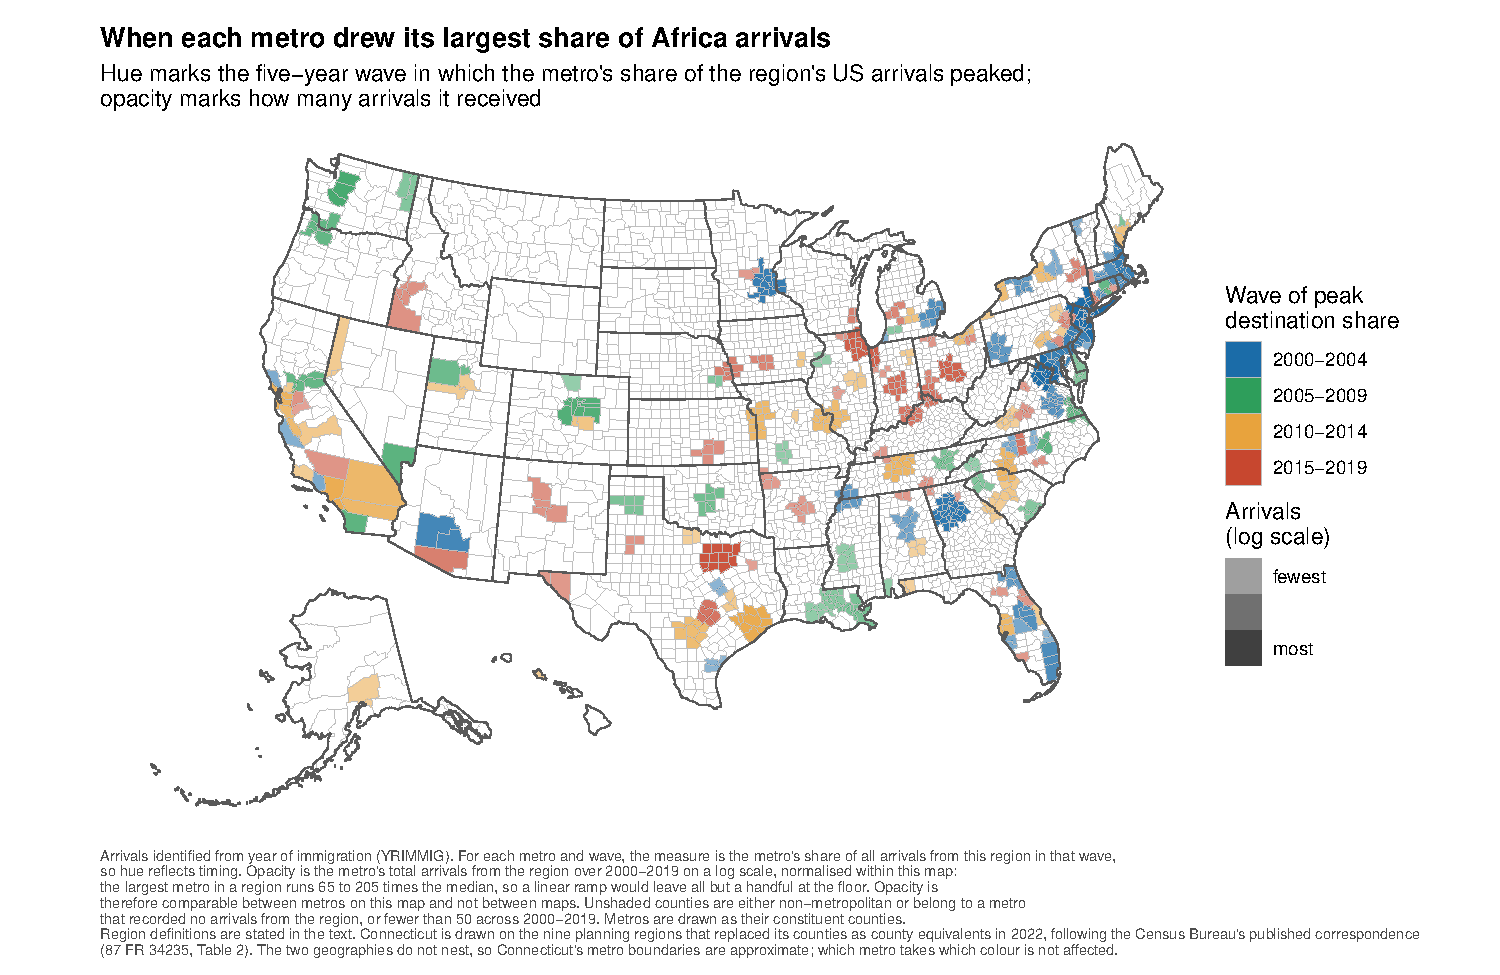
\includegraphics[width=\textwidth]{fig_destination_africa.pdf}
\caption{Metropolitan destinations of African arrivals, by peak five-year wave.
Construction, the treatment of unshaded counties, and the Connecticut and
Puerto Rico notes are as in Figure~\ref{fig:dest_americas}.}
\label{fig:dest_africa}
\end{figure}

\begin{figure}[htbp]
\centering
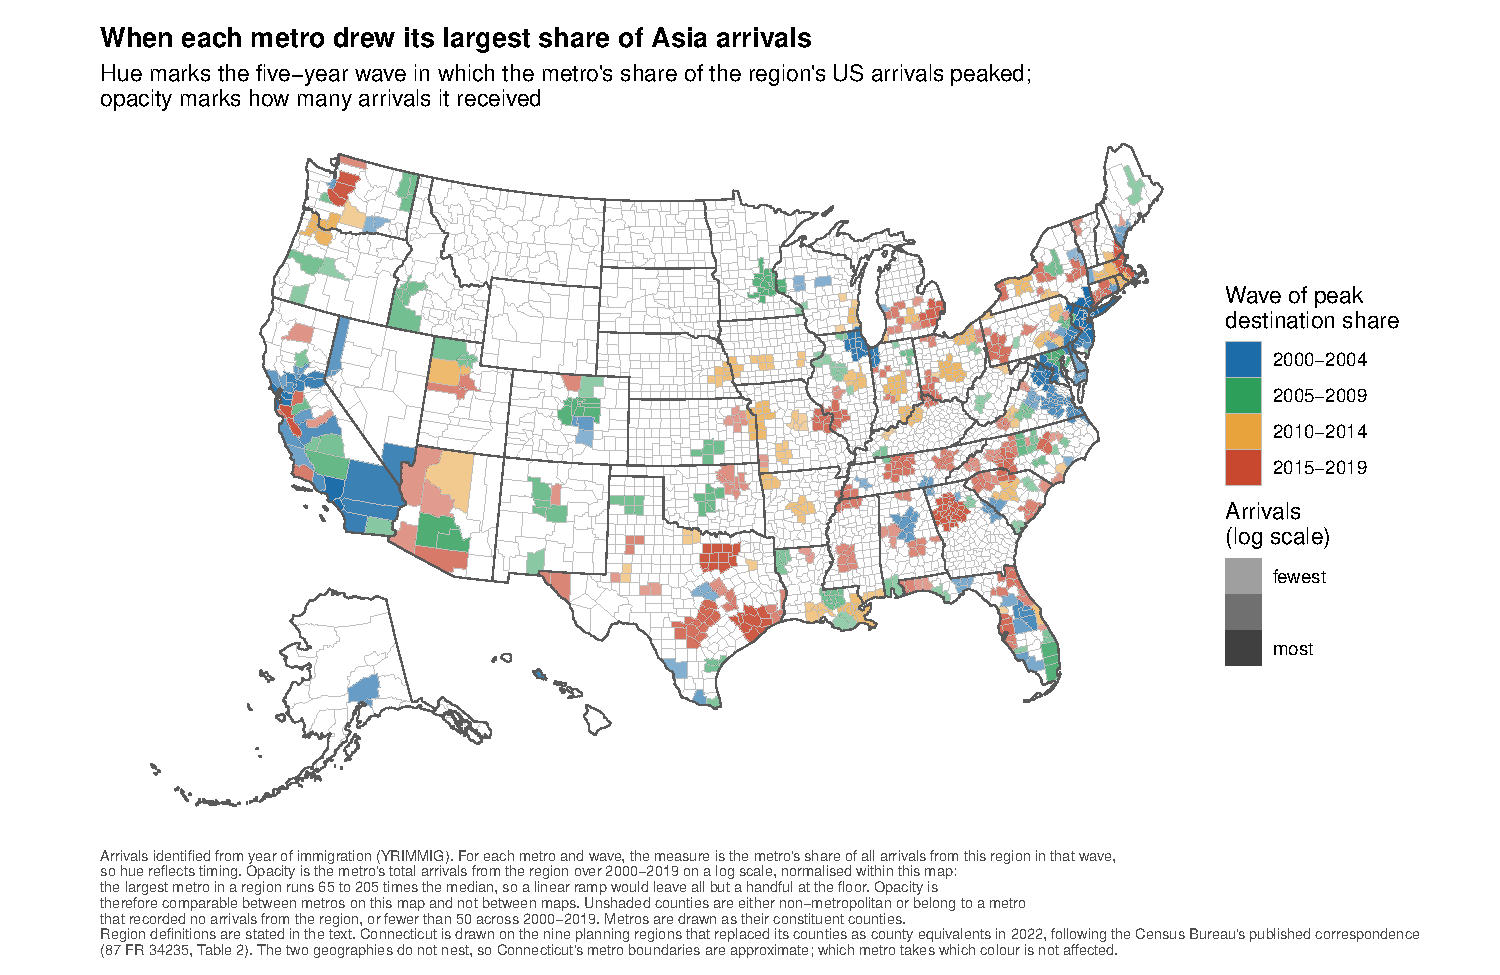
\includegraphics[width=\textwidth]{fig_destination_asia.pdf}
\caption{Metropolitan destinations of Asian arrivals, by peak five-year wave.
Construction, the treatment of unshaded counties, and the Connecticut and
Puerto Rico notes are as in Figure~\ref{fig:dest_americas}.}
\label{fig:dest_asia}
\end{figure}

\begin{figure}[htbp]
\centering
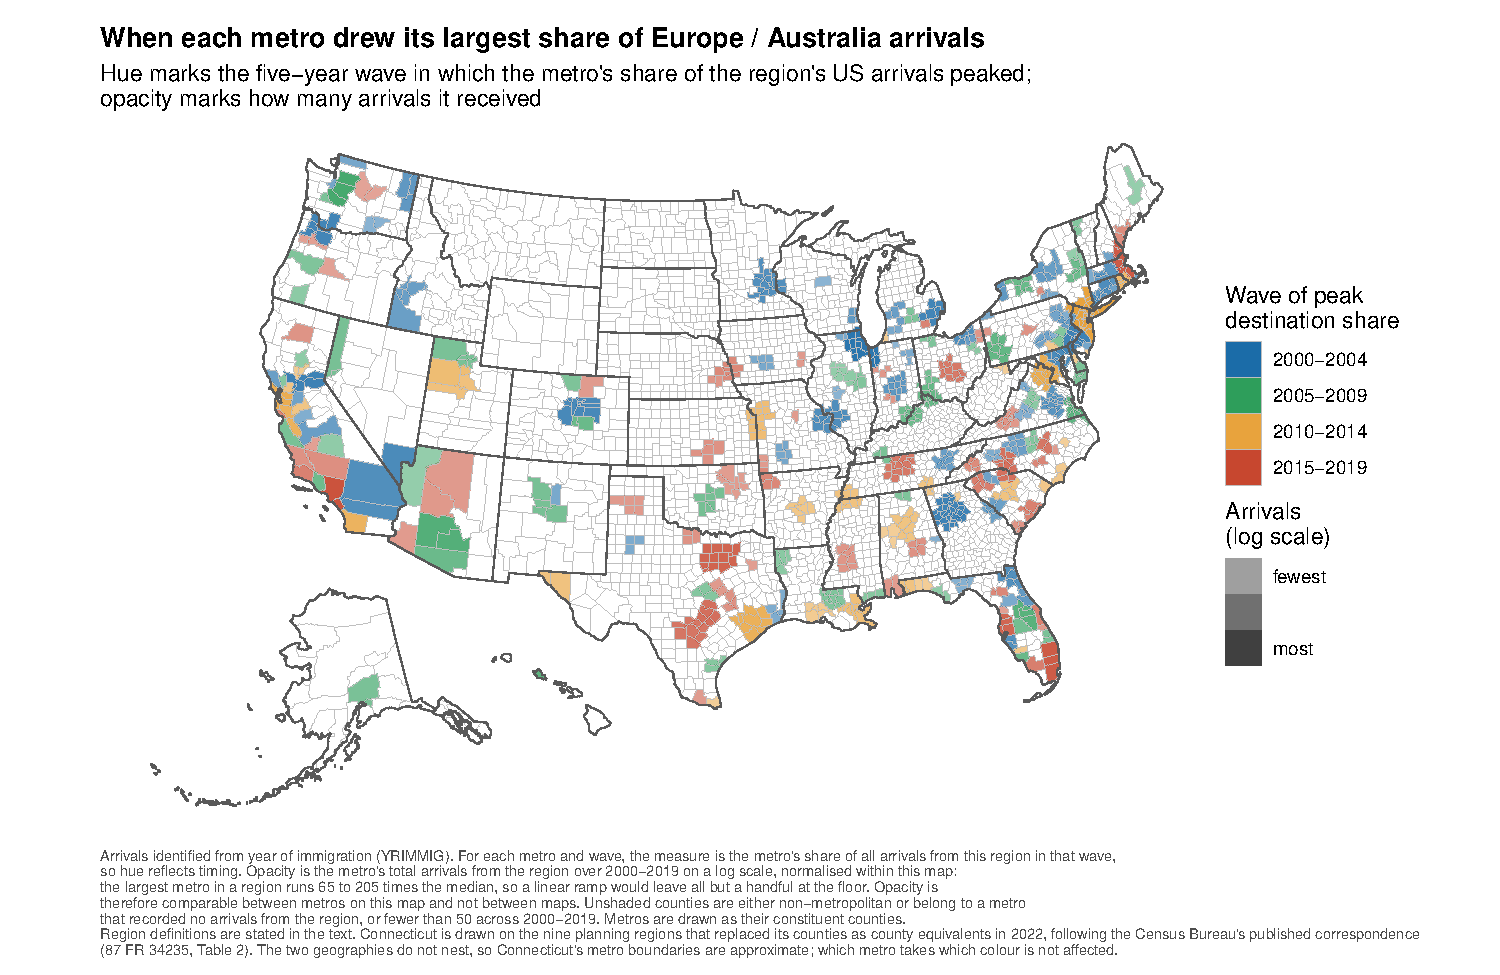
\includegraphics[width=\textwidth]{fig_destination_europe_australia.pdf}
\caption{Metropolitan destinations of European and Australian arrivals, by peak five-year wave.
Construction, the treatment of unshaded counties, and the Connecticut and
Puerto Rico notes are as in Figure~\ref{fig:dest_americas}.}
\label{fig:dest_europe}
\end{figure}

\begin{figure}[htbp]
\centering
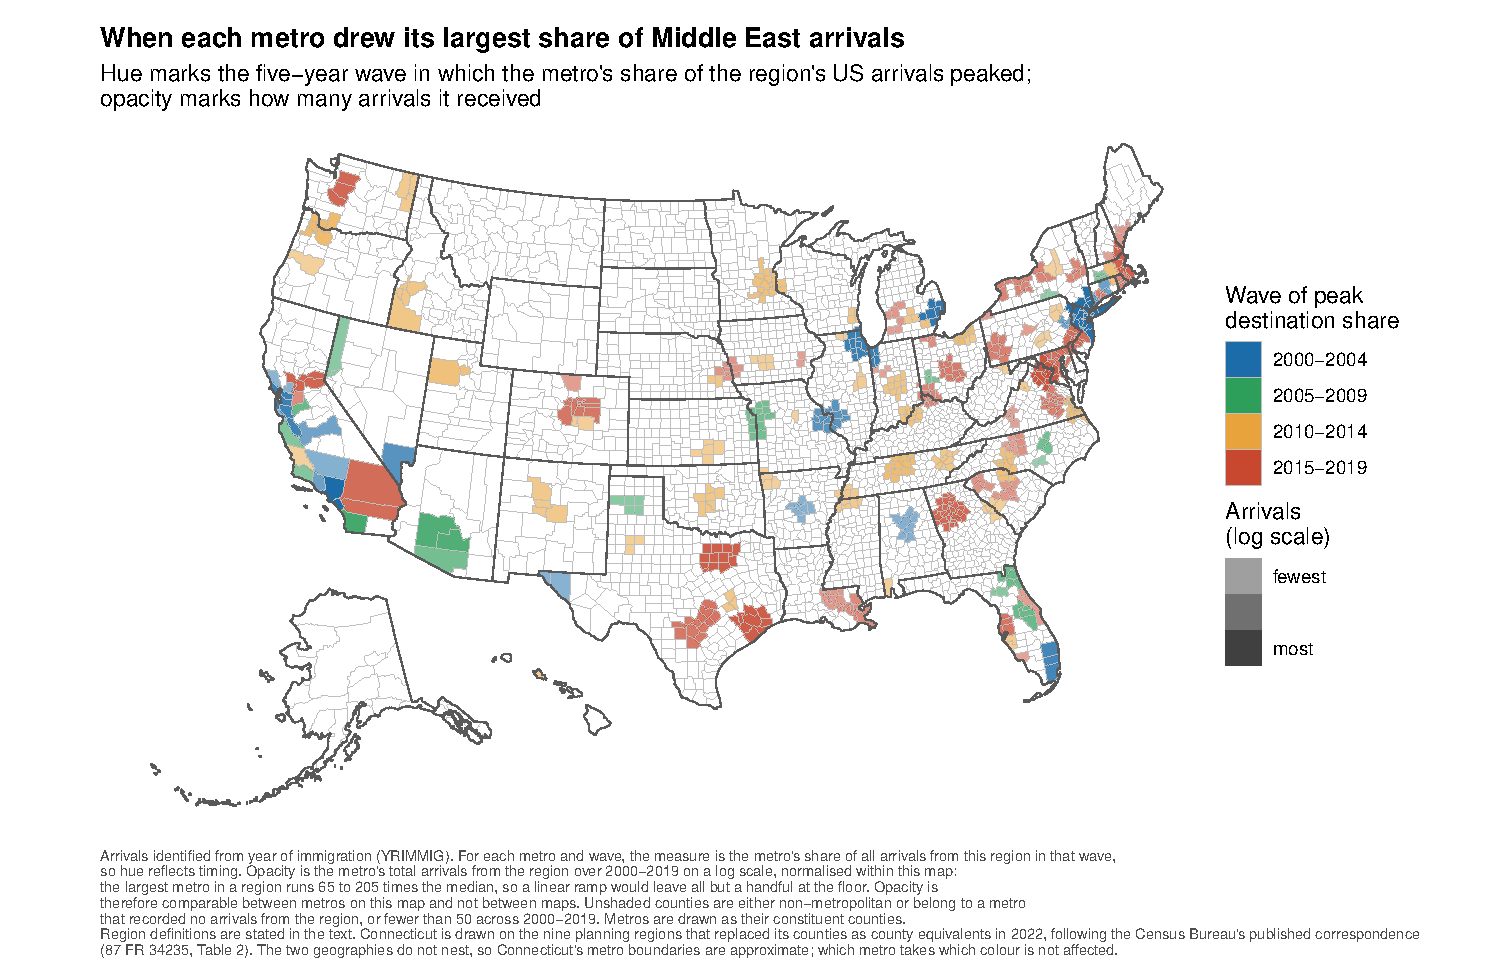
\includegraphics[width=\textwidth]{fig_destination_middle_east.pdf}
\caption{Metropolitan destinations of Middle Eastern arrivals, by peak five-year wave.
Construction, the treatment of unshaded counties, and the Connecticut and
Puerto Rico notes are as in Figure~\ref{fig:dest_americas}.}
\label{fig:dest_mideast}
\end{figure}

% ===========================================================================
\subsection{Education composition of arrivals by age at arrival}
\label{sec:age-sensitivity}
% ===========================================================================

The education composition of immigrant arrivals is not an input to the instrument, which uses arrival counts by origin and not arrival education. It is reported here because the raw series carries an apparent break that invites a reading the data do not support.

Tracking the composition of immigrant arrivals over time reveals a pattern that, absent further scrutiny, would appear directly relevant to the identification strategy (Figure~\ref{fig:educ_prop}). From 1990 through roughly 2005, the share of immigrants with some college or above ($\text{Educ\_Binary} = 1$) declines steadily, while the share without a high school diploma rises over the same period -- notwithstanding that some college remains the plurality education group among immigrants throughout. Beginning around 2005, both trends reverse: the some-college share rises from 2005 to roughly 2015, before declining again toward the end of the sample. The timing of this reversal coincides closely with two federal enforcement developments in 2005. The REAL ID Act of 2005 tightened asylum evidentiary standards and restricted judicial review in removal proceedings, and later that year Operation Streamline -- a joint Department of Homeland Security and Department of Justice enforcement initiative, not a presidential executive order -- shifted the handling of illegal border crossings from civil to criminal proceedings. Either development plausibly contributed to the reversal in both series.

Read on its own, the pattern documented above could be taken as evidence of a genuine, contemporaneous shift in the human capital composition of adult immigrant arrivals coinciding with the 2005 enforcement changes -- a reading that would carry direct implications for the exposure measure developed below, since a real shift in the composition of the adult population supplying that exposure would itself be a potential confound rather than a benign feature of the data. This reading does not survive disaggregation by age at arrival. Restricting the sample to individuals aged 25 and older removes the apparent break entirely (Figure~\ref{fig:educ_prop_25plus}): across the full sample period, the some-college share among immigrants aged 25 and older rises in an almost monotonic fashion, and the no-high-school share falls almost monotonically, with no visible discontinuity around 2005. By contrast, restricting to immigrants aged 18--24 at arrival reproduces a sharp inflection at 2005 (Figure~\ref{fig:educ_prop_1824}): the some-college share, which fluctuates in a relatively narrow band (roughly 37--44 percent) from 1990 through 2005, begins a sustained rise immediately afterward, reaching roughly 64 percent by 2011 and remaining elevated through the mid-2010s before declining toward the end of the sample; the no-high-school share among this age group shows the mirror-image pattern, falling sharply over the same window.

Taken together, these three versions of the same underlying figure (Figures~\ref{fig:educ_prop}, \ref{fig:educ_prop_25plus} and \ref{fig:educ_prop_1824}) indicate that the apparent 2005 break in the full, age-unrestricted sample is driven primarily by a shift in the age composition of immigrant arrivals rather than by a change in the education composition of the adult immigrant population per se. The share of arrivals under 18 appears to have been rising from 1990 to 2005, inflating the no-high-school share mechanically, since school-age arrivals have not yet had the opportunity to complete their schooling; consequently, the post-2005 reversal in the unrestricted figure is better understood as a shift specifically among young adult arrivals (ages 18--24) than as a broad-based change across the full immigrant population. This distinction matters beyond descriptive accuracy: it determines which population the subsequent education-composition results should be read as characterizing, and forecloses a reading of the raw series that would otherwise misattribute a compositional artifact to a genuine shift in immigrant human capital.\footnote{This age-at-arrival sensitivity is a distinct issue from the birth-cohort concern raised above in connection with the exposure measure. The age-at-arrival pattern here concerns how the raw descriptive composition of immigrant arrivals is measured across ages; the birth-cohort concern concerns whether the identifying variation in the shift-share instrument is confounded with secular trends in national immigrant inflows once the exposure window is fixed by birth year. The two should not be conflated: resolving the former, as this subsection does, does not bear on the latter, which is addressed separately in the robustness discussion.}

\begin{figure}[htbp]
\centering
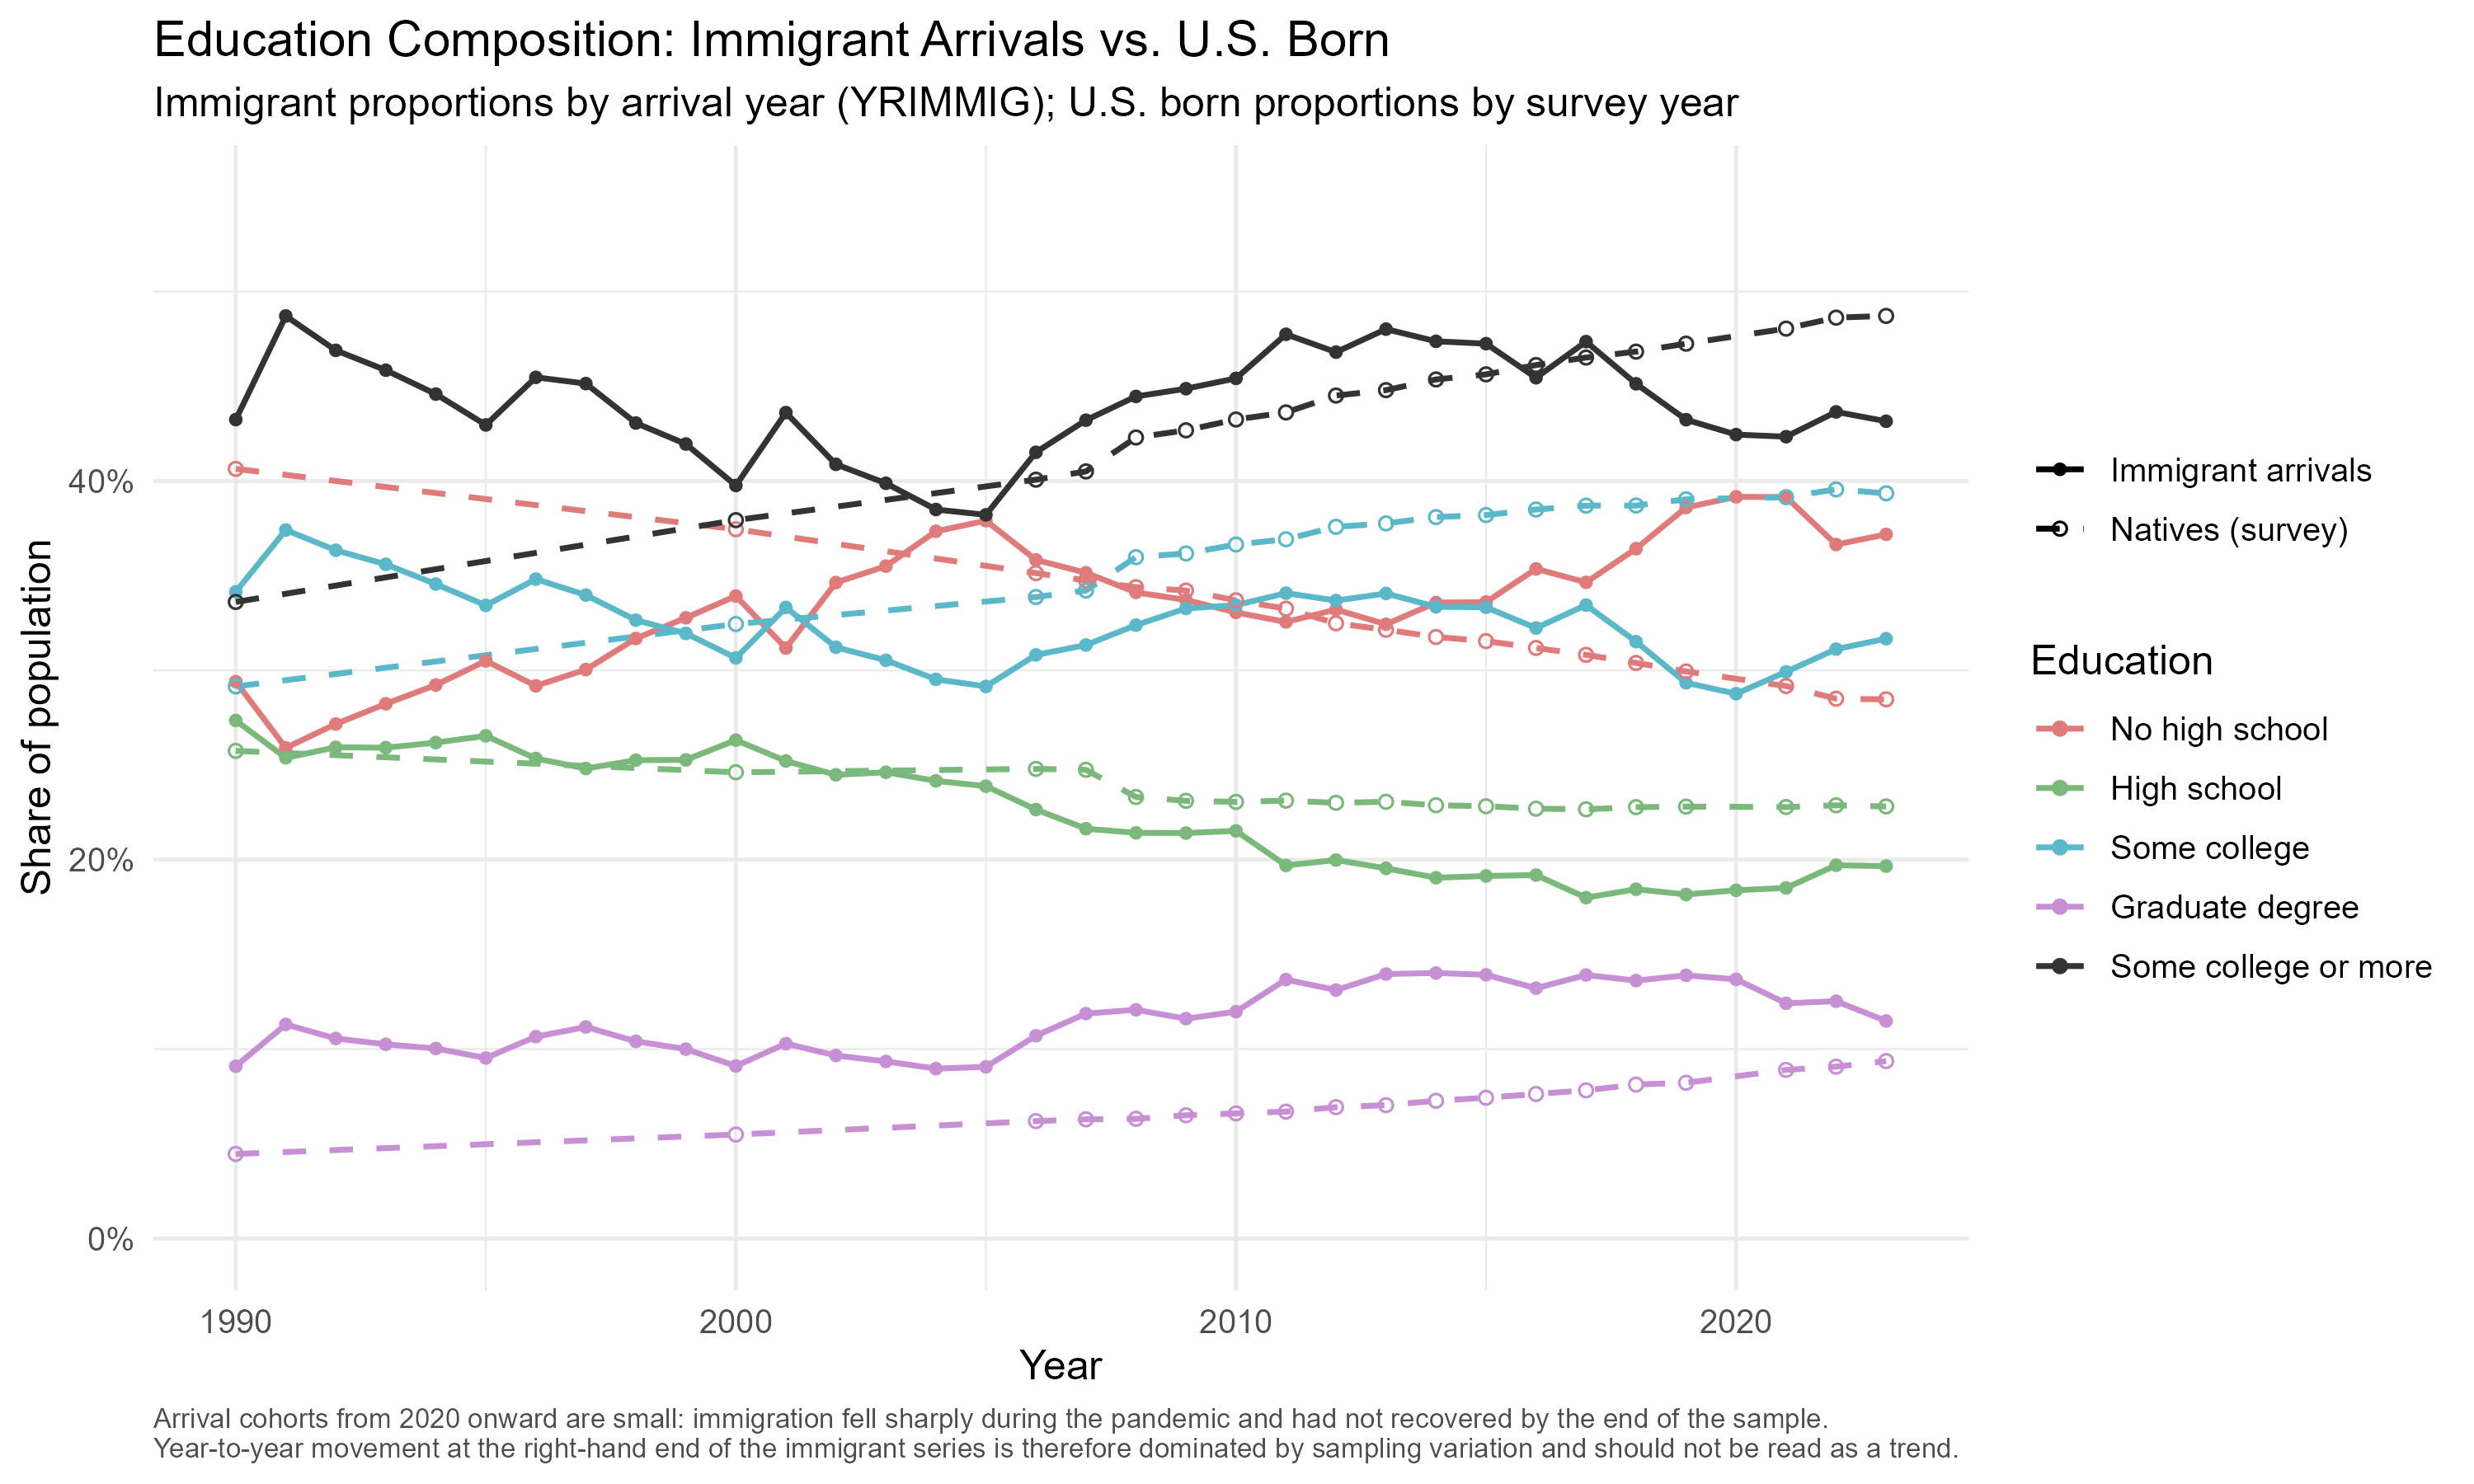
\includegraphics[width=\textwidth]{Educ_Prop.png}
\caption{Education composition of immigrant arrivals by year of arrival,
1990--2023, all ages at arrival. Shares are population-weighted using IPUMS
person weights and sum to one within each arrival year. Educational
attainment is measured at the survey date rather than at arrival, so recent
arrival cohorts have had less time to complete schooling in the United
States. No observations exist for 2001--2005, where the panel moves from the
2000 decennial census to the 2006 ACS; the series should be read as absent
across that window rather than interpolated through it. Arrival cohorts from
2020 onward are small, immigration having fallen sharply during the pandemic
and not recovered by the end of the sample, so year-to-year movement at the
right-hand end of the immigrant series reflects sampling variation rather
than a change in composition.}
\label{fig:educ_prop}
\end{figure}

\begin{figure}[htbp]
\centering
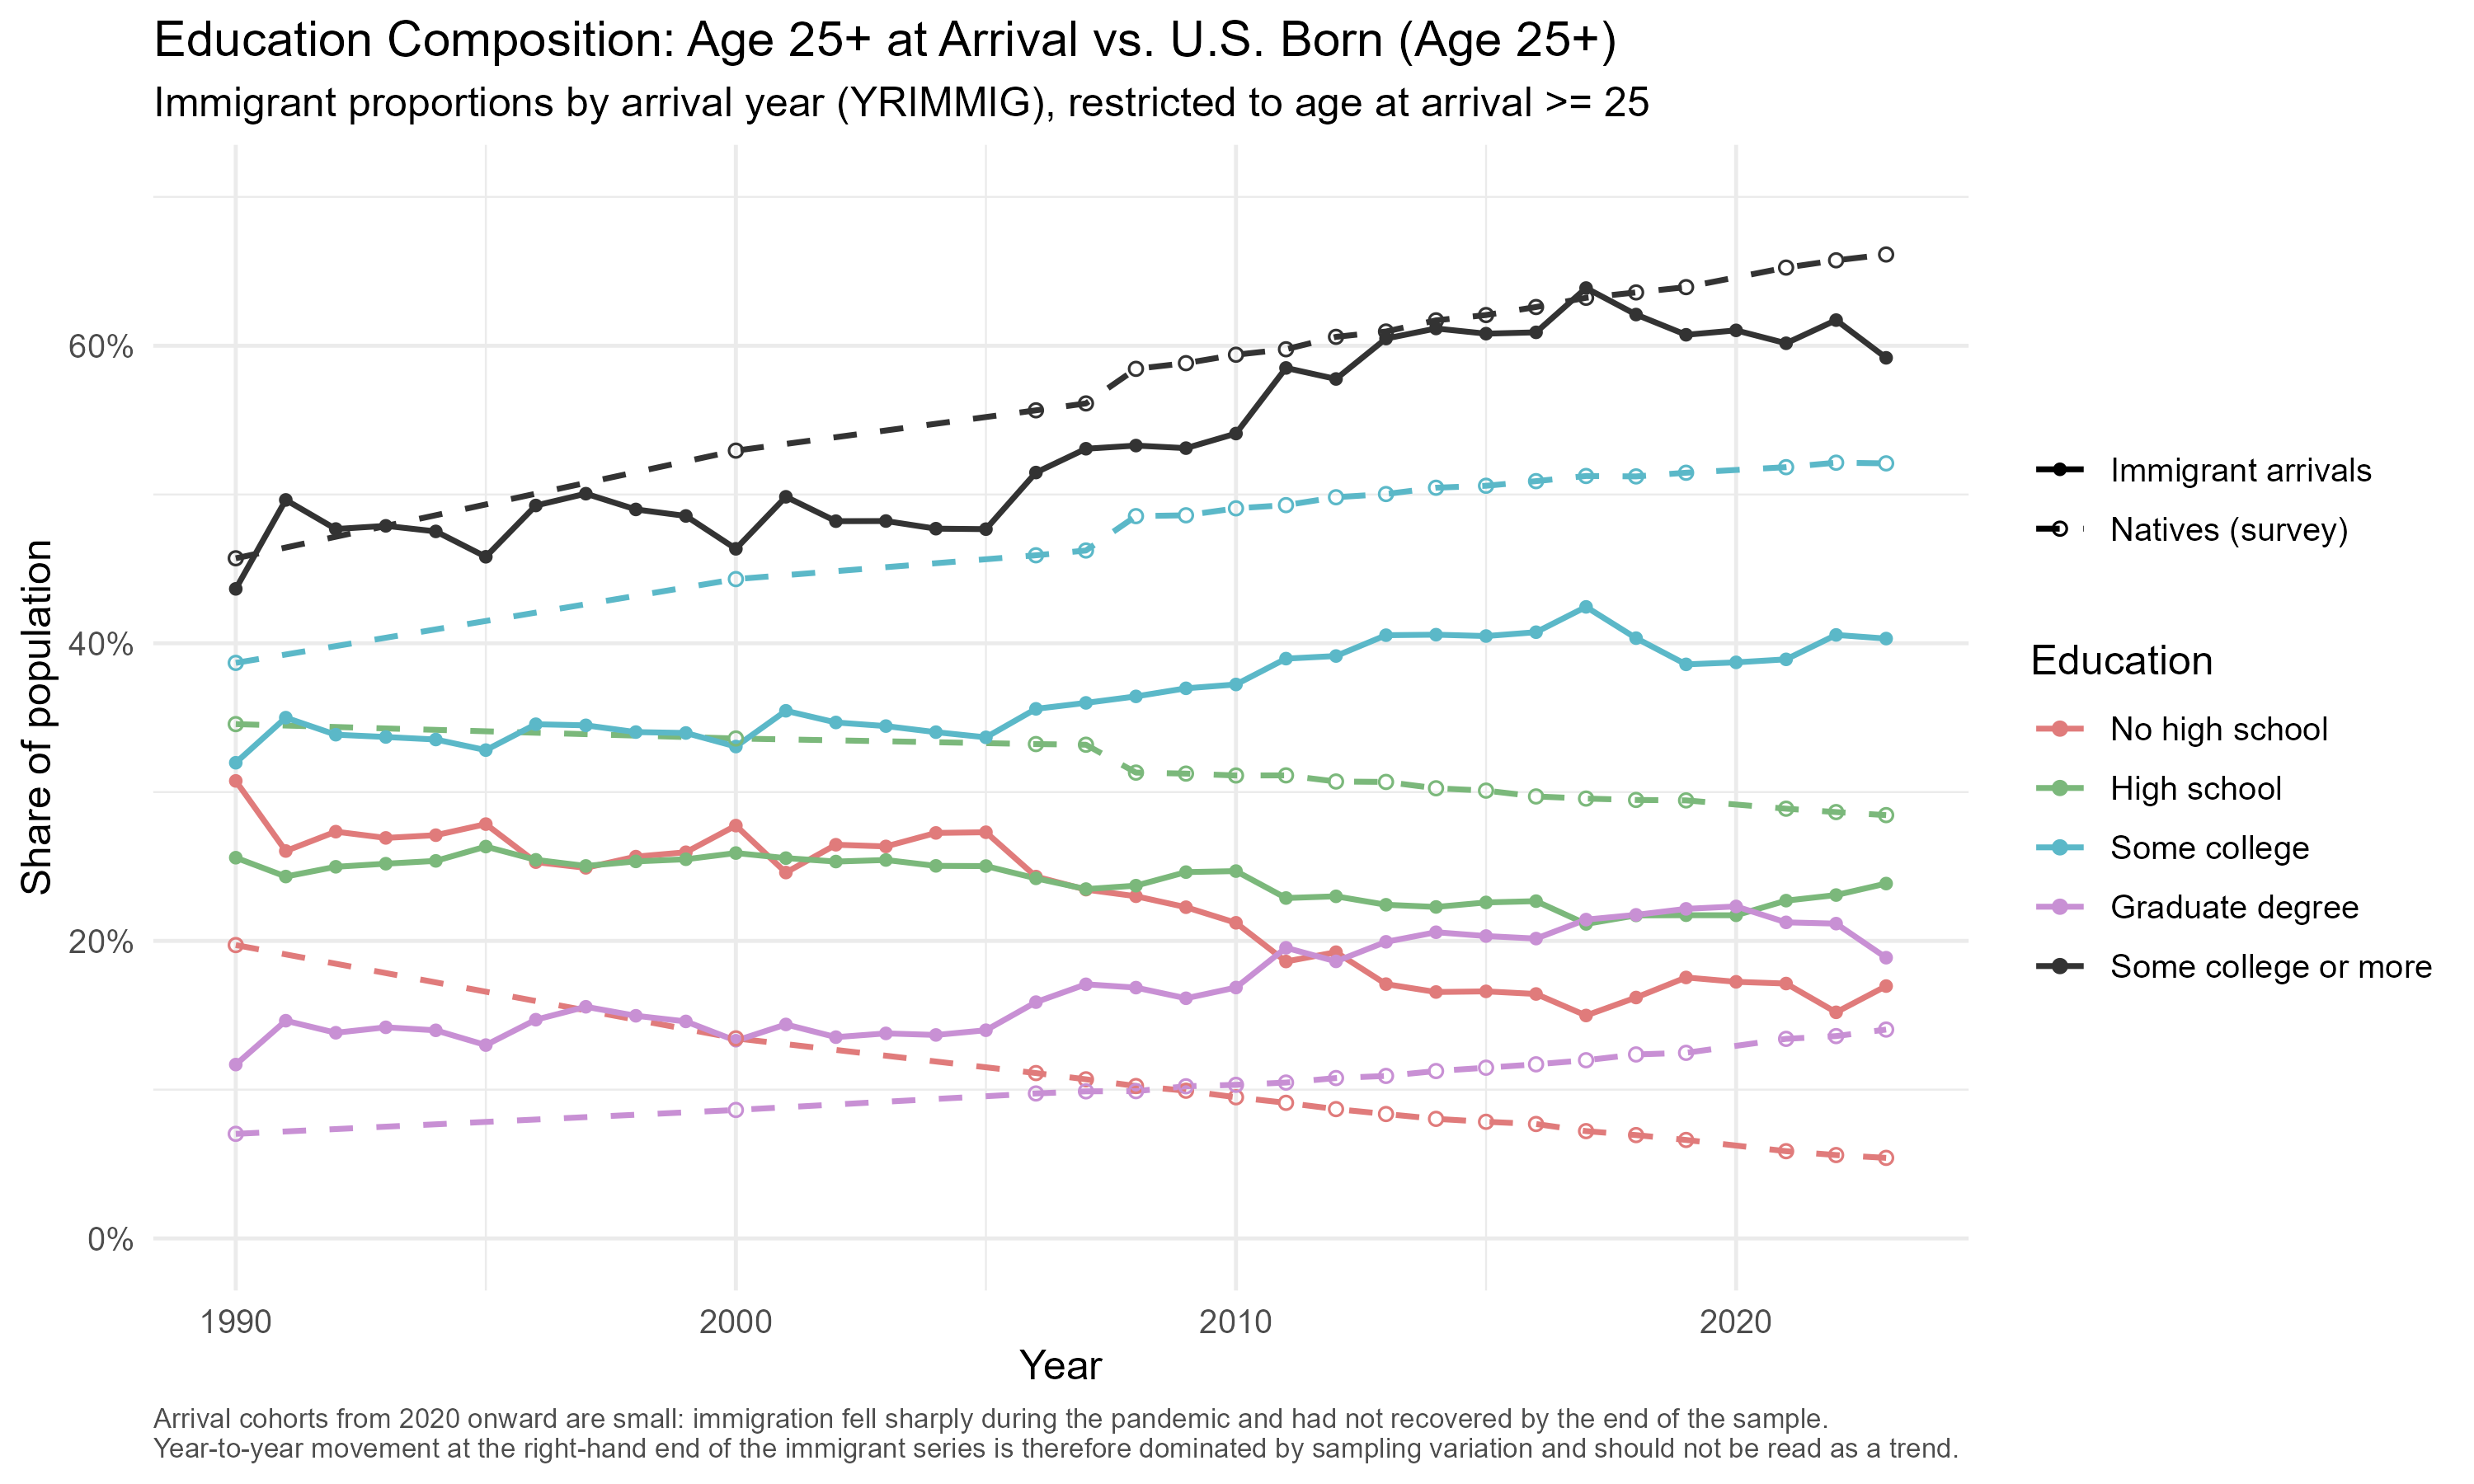
\includegraphics[width=\textwidth]{Educ_Prop_Age25plus.png}
\caption{Education composition of immigrant arrivals aged 25 and older at
arrival, 1990--2023. Restricting to arrivals who had reached the
conventional age for completed schooling removes the 2005 break visible in
Figure~\ref{fig:educ_prop}: the some-college-or-above share rises almost
monotonically across the full period and the no-high-school share falls
almost monotonically. Construction, weighting, the 2001--2005 gap and the
caveat on post-2020 arrival cohorts are as in Figure~\ref{fig:educ_prop}.}
\label{fig:educ_prop_25plus}
\end{figure}

\begin{figure}[htbp]
\centering
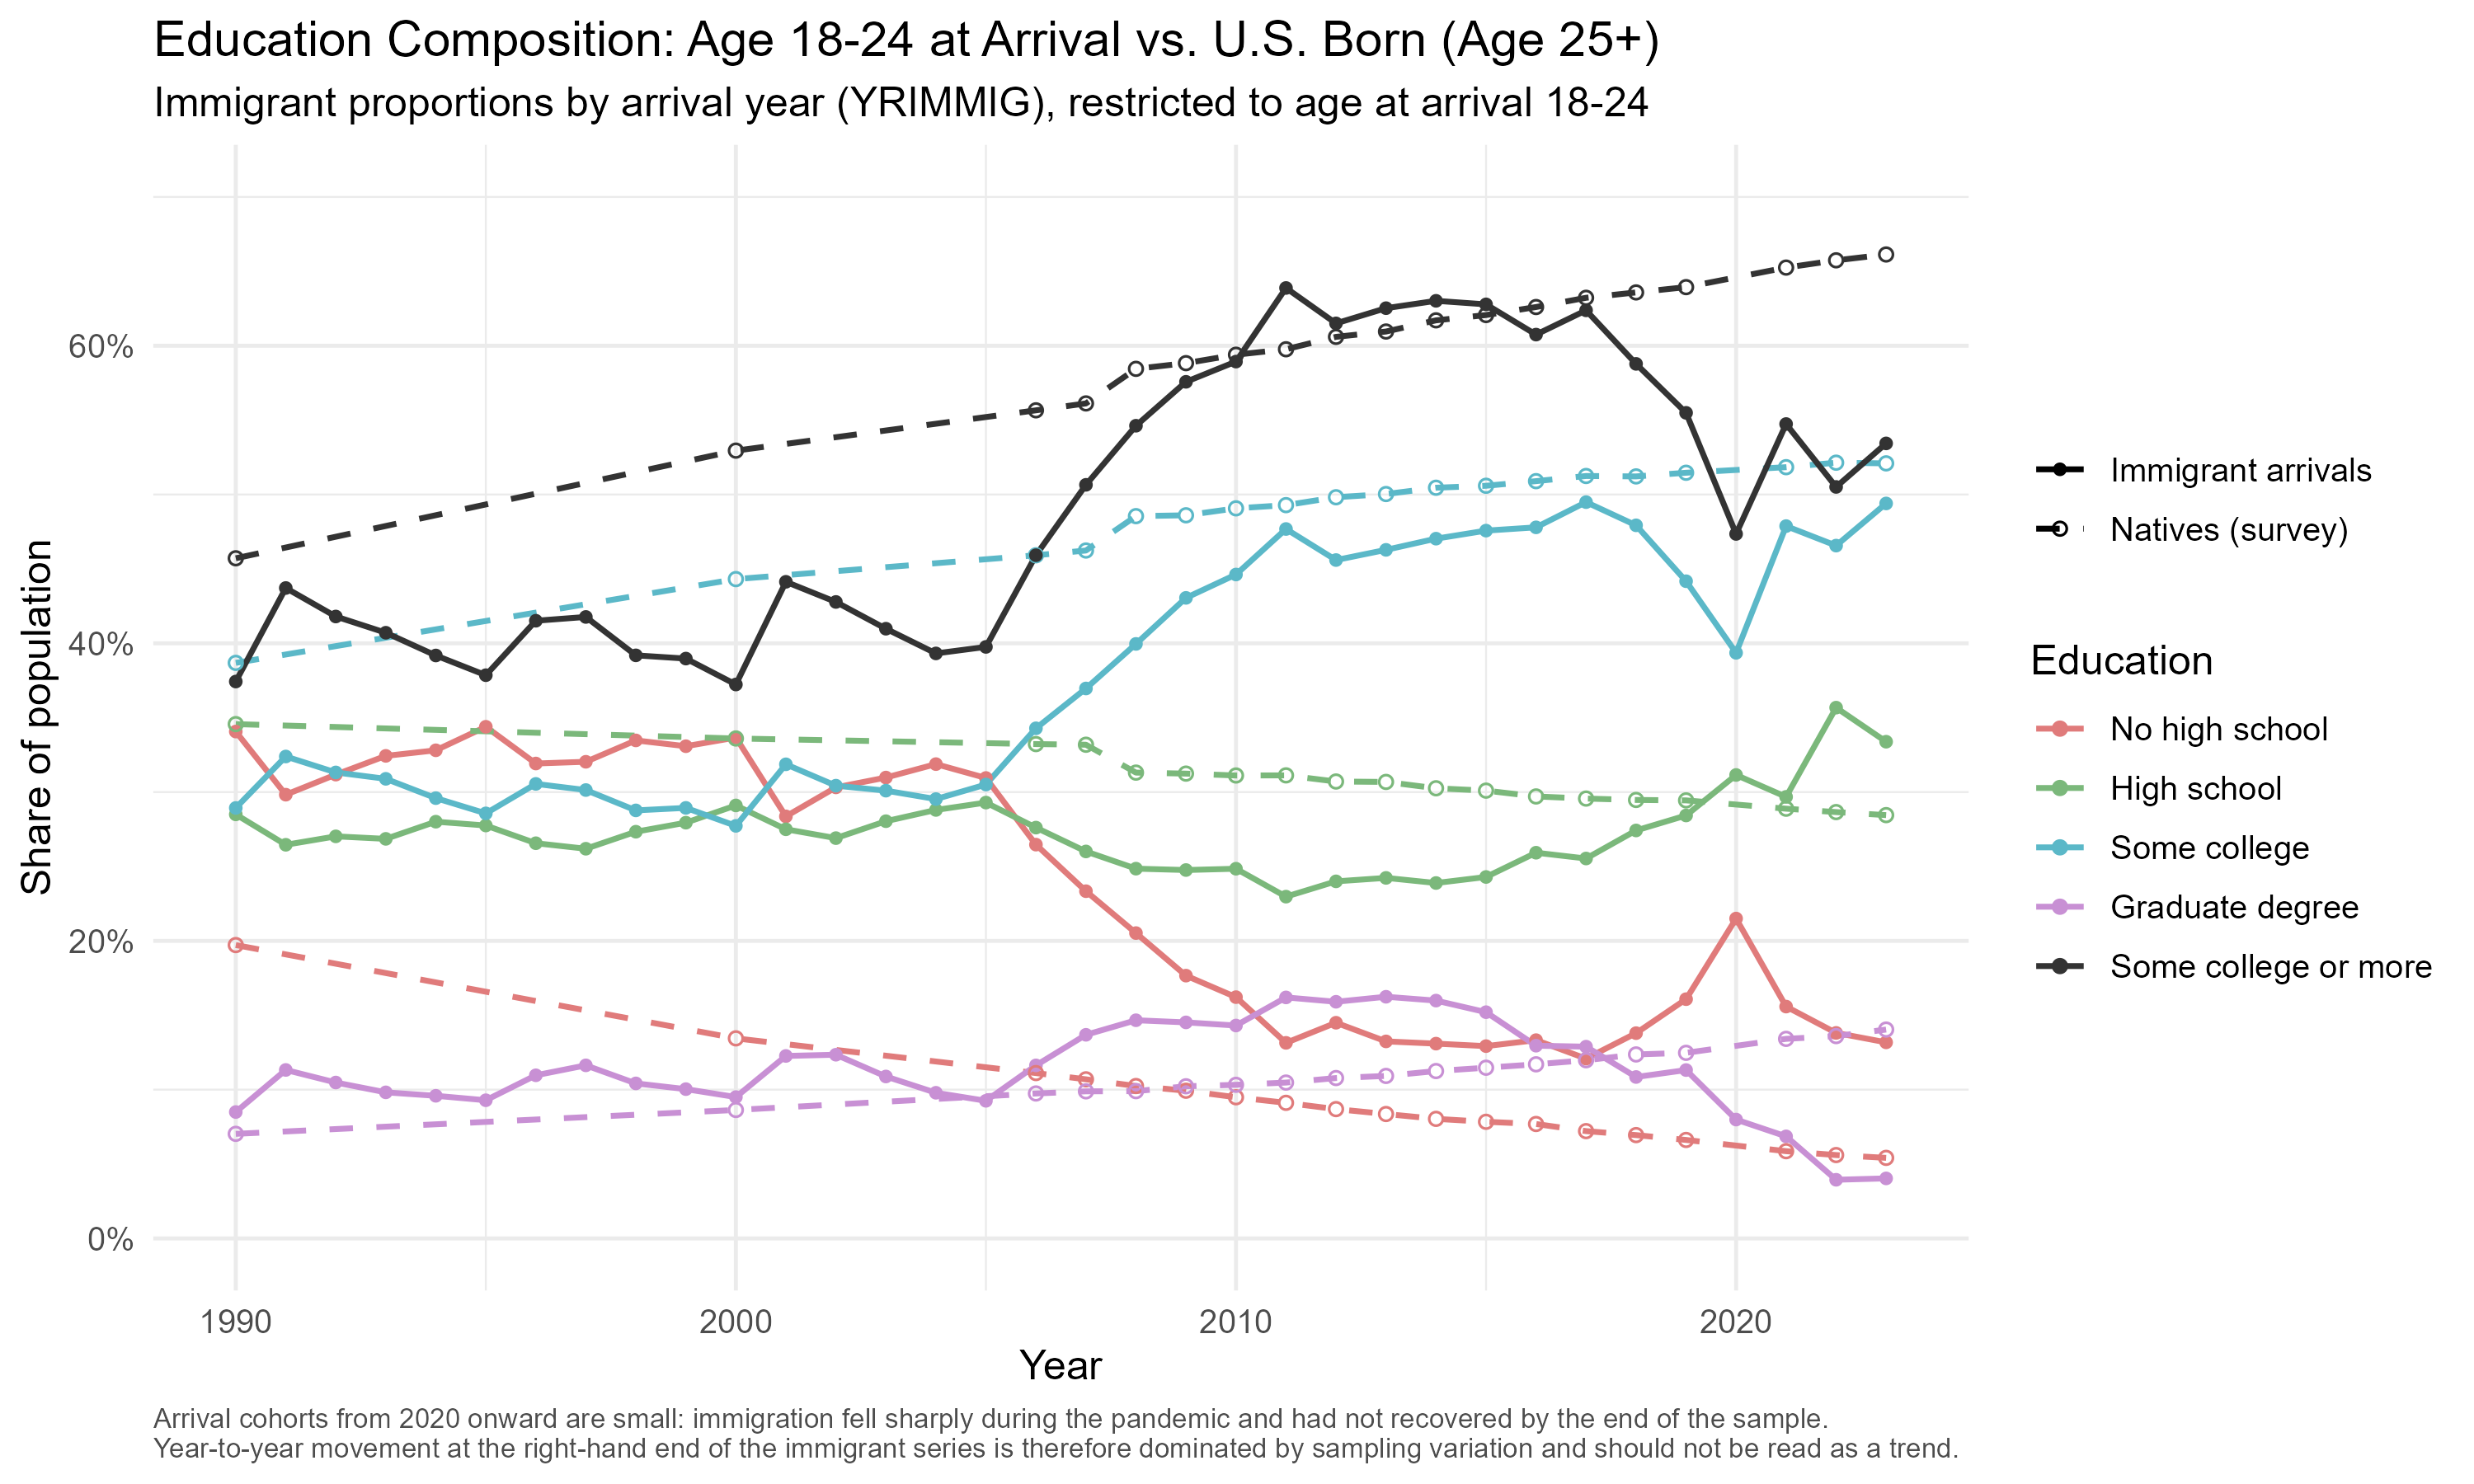
\includegraphics[width=\textwidth]{Educ_Prop_Age18to24.png}
\caption{Education composition of immigrant arrivals aged 18--24 at arrival,
1990--2023. This age group reproduces the 2005 inflection in sharp form: the
some-college-or-above share holds within roughly 37--44 percent from 1990
through 2005, then rises to roughly 64 percent by 2011, with the
no-high-school share tracing the mirror image. Read alongside
Figure~\ref{fig:educ_prop_25plus}, the contrast locates the break in the
changing age composition of arrivals rather than in the education
composition of the adult immigrant population. Construction, weighting, the
2001--2005 gap and the caveat on post-2020 arrival cohorts are as in
Figure~\ref{fig:educ_prop}.}
\label{fig:educ_prop_1824}
\end{figure}


% ===========================================================================
% ===========================================================================
\bibliographystyle{aea}
\bibliography{bibliography}

\end{document}
